%Nicht anfassen, so ist der Dokumentenaufbau
\documentclass[a4paper, 12pt]{article}
\usepackage[utf8]{inputenc} % Kodierung
\usepackage[T1]{fontenc} % Explizite Nennung des Fonts
% Use Times-like font (text + math)
\usepackage{newtxtext,newtxmath}
\usepackage[ngerman]{babel} % Sprache (Deutsch)
\usepackage{graphicx} % immer benötigt für das Einbinden von Graphiken
\usepackage{blindtext} % Wenn man das Layout prüfen will, kann hier mit \blindtext Text eingfügt werden.
%\usepackage{parskip} % Für den Abstand zwischen 2 Absätzen.
%\setlength{\parskip}{7pt plus20pt minus10pt} % Genaue Einstellung von parskip
\usepackage{subcaption}
\usepackage{easy-todo} % Mit \todo{} Todos einfügen
\usepackage{csquotes} % Für ordentlichen Anführungszeichen
\usepackage[iso, ngerman]{isodate} % Deutsche Datumsformatierung
\usepackage[style=apa, 
backend=biber, 
bibencoding=utf8, 
language=ngerman, 
mincitenames=1, 
maxcitenames=2]{biblatex}
\addbibresource{literatur/bibliography.bib} % Einbinden der Literatur.
\AtEveryBibitem{\clearfield{annotation}} % Unterdrückt "Article." aus den annote-Feldern der .bib-Datei
\usepackage{amsmath}

\DefineBibliographyStrings{ngerman}{%
  urlseen = {Abgerufen am},
  % APA verlangt "et al." statt der deutschen Abkuerzung "u. a."
  andothers = {et\addabbrvspace al\adddot},
}

\DeclareLanguageMapping{ngerman}{ngerman-apa} % Bibliographie-Sprache fuer APA
\usepackage{float} % Grafik bleibt dort wo man sie im Code platziert hat

\usepackage[activate={true,nocompatibility},
	final,
	tracking=true,
	kerning=true,
	expansion=true,
	spacing=true,
	factor=1050,
	stretch=25,
	shrink=10]{microtype} % Für die Feineinstellung der Zeichensetzung.
\usepackage{booktabs}
\usepackage{appendix}
\usepackage[rflt]{floatflt}
\usepackage{fancyvrb}
\usepackage[hidelinks]{hyperref} % Klickbare aber nicht markierte Links im PDF
\usepackage{setspace}
\usepackage{fancyhdr} % Für schönere Kopf-/Fußzeilen und Fußnoten.
\usepackage[left=3cm, right=2cm, top=2.5cm, bottom=2cm]{geometry} % Seitenränder
\usepackage{pbox}
\usepackage{tabulary}
\usepackage{outlines}
\usepackage{matlab-prettifier}
\usepackage{listings}
\usepackage{color} %red, green, blue, yellow, cyan, magenta, black, white

% Für die Abbildung
\usepackage{tikz}
\usepackage{pgfplots}
\pgfplotsset{width=0.7*\textwidth,compat=1.9}

% Für Tabellen
\usepackage{csvsimple}
\usepackage{longtable}
\usepackage{rotating}
\usepackage{pdflscape} % Querformat-Seiten (inkl. gedrehter Überschrift)
\usepackage{multirow}

\definecolor{mygreen}{RGB}{28,172,0} % color values Red, Green, Blue
\definecolor{mylilas}{RGB}{170,55,241}

%Kein Schusterjunge/Hurenkind im Text
\widowpenalty10000
\clubpenalty10000
\usepackage[justification=centering]{caption}

\usepackage{titlesec}

% --- Formatierung für \section ---

% Aussehen der Überschrift
\titleformat{\section}
  {\normalfont\LARGE\bfseries} % Hier die Größe anpassen (z. B. \Large, \LARGE, \huge)
  {\thesection}                % Die Nummerierung (z.B. "1")
  {1em}                        % Abstand zwischen Nummerierung und Text
  {}                           % Zusätzlicher Code vor der Überschrift (hier leer)

% Abstände der Überschrift
\titlespacing*{\section}
  {0pt}      % Einzug von links
  {18pt}     % Abstand nach oben (vor der Überschrift)
  {18pt}     % Abstand nach unten (nach der Überschrift)
  \titlespacing*{\subsection}
  {0pt}      % Einzug von links
  {12pt}     % Abstand nach oben (vor der Überschrift)
  {12pt}     % Abstand nach unten (nach der Überschrift)
% Aussehen der \paragraph-Ueberschrift (eigene Zeile statt Fliesstext)
\titleformat{\paragraph}[hang]
  {\normalfont\normalsize\bfseries}
  {\theparagraph}
  {1em}
  {}
\titlespacing*{\paragraph}
  {0pt}
  {10pt}
  {6pt}

% Abstand ueber und unter abgesetzten Formeln.
% Standard sind 12pt ueber und unter dem Block, waehrend einzelne Gleichungen nach
% einer kurzen Zeile mit \abovedisplayshortskip = 0pt gesetzt werden. Dadurch stehen
% align-Bloecke deutlich lockerer als \begin{equation}. Die Werte unten gleichen das an.
% \normalsize setzt die Laengen bei jedem Schriftgroessenwechsel auf die Klassenwerte
% zurueck, deshalb werden sie dort angehaengt.
\makeatletter
\newcommand{\FormelAbstaende}{%
  \setlength{\abovedisplayskip}{5pt plus 2pt minus 2pt}%
  \setlength{\belowdisplayskip}{8pt plus 2pt minus 3pt}%
  \setlength{\abovedisplayshortskip}{6pt plus 2pt minus 1pt}%
  \setlength{\belowdisplayshortskip}{8pt plus 2pt minus 3pt}%
}
\g@addto@macro\normalsize{\FormelAbstaende}
\makeatother
\AtBeginDocument{\FormelAbstaende}

% Note: removed \sloppy to preserve proper hyphenation and justification
\fancyhf{}
\cfoot{\thepage}
\renewcommand{\headrulewidth}{0pt}
%Special cells with linebreaks possible
\newcommand{\specialcell}[2][c]{%
	\begin{tabular}[#1]{@{}t@{}}#2\end{tabular}}
%define blockquote-quotation environment
\renewenvironment{quotation}{
	\leftskip1cm
	\rightskip1cm
	\noindent
	\setstretch{1}
	\small
}

% define Footnote
\renewcommand\footnoterule{\kern-3pt \hrule width 3in height 0.7pt \hskip3pt \kern 2.6pt}
\let\oldfootnote\footnote
\renewcommand\footnote[1]{%
	\oldfootnote{\hspace{2mm}#1}}
%%%%%

% microtyping around some characters

%Extra-spacing around dash, and quotation-marks, and parentheses
\SetExtraKerning[unit=space]
	{
		encoding={*}, family={qhv}, series={b}, size={normalsize,large,Large}
	}
	{
		\textendash={400,400}, % for double-dash
		\textquotedblleft={ ,120}, % for left quotation-mark
		\textquotedblright={170, }, % for right quotation-mark
		"28={ ,250}, % left bracket, add space from right
		"29={300, } % right bracket, add space from left
	}

%%%%%


\makeatletter
\newcommand{\MSonehalfspacing}{%
  \setstretch{1.44}%  default
  \ifcase \@ptsize \relax % 10pt
    \setstretch {1.448}%
  \or % 11pt
    \setstretch {1.399}%
  \or % 12pt
    \setstretch {1.433}%
  \fi
}
\newcommand{\MSdoublespacing}{%
  \setstretch {1.92}%  default
  \ifcase \@ptsize \relax % 10pt
    \setstretch {1.936}%
  \or % 11pt
    \setstretch {1.866}%
  \or % 12pt
    \setstretch {1.902}%
  \fi
}
\newcommand{\MSverbatimspacing}{%
  \setstretch{1.44}%  default
  \ifcase \@ptsize \relax % 10pt
    \setstretch {1}%
  \or % 11pt
    \setstretch {1}%
  \or % 12pt
    \setstretch {1}%
  \fi
}
\makeatother

\begin{document}
\newgeometry{margin=2.5cm}
\begin{titlepage}
\thispagestyle{empty}
% Deckblatt zaehlt als Seite 0 und damit nicht mit
\setcounter{page}{0}
\newcommand{\HRule}{\rule{\linewidth}{0.5mm}}
\hspace{1cm}
\center

\textsc{\huge Universität Bremen}\\[1.6cm]
\textsc{\Large Fachbereich 07 -- Wirtschaftswissenschaften}\\[0.8cm]
\MSonehalfspacing
\textsc{\Large Hausarbeit}\\[0.8cm]

\HRule\\[1cm]
\MSdoublespacing
{ \huge \bfseries Risikobasierte Portfoliooptimierung mit GARCH-Modellen}\\[0.2cm]
\HRule \\[0.8cm]
\MSonehalfspacing

	\begin{tabular}{ll}
		\large{Verfasser:}		& \large{Simon Johannes Jähn} \\
		& \normalsize{jaehn1@uni-bremen.de} \\
		& 6186771 \\[0.3cm]
		& \large{Angela Nikoyan}
		\vspace{0.6cm}\\
			\large{Veranstaltung:}	& \large{Portfoliotheorie und Asset Management} \\
		& \normalsize{07-M37-4-02-01}
		\vspace{0.6cm}\\
			\large{Dozent:}		& \large{Prof. Dr. Thorsten Poddig}
		\vspace{0.6cm}\\
			\large{Studiengang:}		& \large{Master Betriebswirtschaftslehre}
		\vspace{0.6cm}\\
			\large{Abgabedatum:}		& \large{\ifnum\day<10 0\fi\the\day.\ifnum\month<10 0\fi\the\month.\the\year}
	\end{tabular}


\end{titlepage}
\restoregeometry

% Das Deckblatt zaehlt nicht mit. Die roemische Nummerierung beginnt erst hier,
% sodass das Inhaltsverzeichnis Seite I ist (\pagenumbering setzt den Zaehler auf 1).
\pagenumbering{Roman}
\pagestyle{fancy}

\setstretch{1.3}
\microtypesetup{protrusion=false}
\setcounter{tocdepth}{2}
\tableofcontents
\addtocontents{toc}{\protect\enlargethispage*{\baselineskip}}

\newpage
\addcontentsline{toc}{section}{\listfigurename}
\listoffigures

\newpage
\addcontentsline{toc}{section}{\listtablename}
\listoftables
\microtypesetup{protrusion=true}

\MSonehalfspacing
\newpage
% Ab hier arabische Nummerierung, beginnend bei 1
\pagenumbering{arabic}

\setcounter{page}{1}
%%%%%%%%%%%%%%%%%%%%%%%%%%%%%
%%%Ab hier Inhalt einfügen%%%
%%%%%%%%%%%%%%%%%%%%%%%%%%%%%

\renewcommand{\abstractname}{Abstrakt}
\begin{abstract}
Diese Arbeit untersucht, ob risikobasierte Portfolioverfahren das naive 1/N-Portfolio schlagen und ob GARCH- und DCC-GARCH-Prognosen der Kovarianzmatrix gegenüber einer historischen Schätzung einen Mehrwert stiften.
Die Grundlage bilden tägliche Renditen von 27~US-Sektorindizes über gut 27~Jahre, die in zehn Trainingsfenstern und vier Prognosehorizonten und damit in 40~Konstellationen ausgewertet werden.
Bewertet wird getrennt nach statistischen und ökonomischen Kriterien.
Statistisch fällt das Ergebnis eindeutig aus, da DCC-GARCH die Kovarianzmatrix unter dem primären QLIKE-Kriterium in 37 und unter dem MSE in allen 40~Konstellationen besser prognostiziert als die historische Matrix.
Ökonomisch schlägt sich dieser Vorsprung allenfalls beim Minimum-Varianz-Portfolio nieder, während er bei Hierarchical Risk Parity und Equal Risk Contribution folgenlos bleibt.
Belastbar ist er jedoch auch dort nicht, da sämtliche Tests auf Sharpe-Differenzen insignifikant ausfallen.
Ausschlaggebend ist der Turnover, der beim Minimum-Varianz-Portfolio mit dynamischer Kovarianz um den Faktor~32 höher liegt und die dynamischen Varianten unter realen Handelskosten zusätzlich belasten würde.
Eine bessere Risikoprognose ist folglich nicht automatisch eine bessere Anlageentscheidung.
Code und Daten liegen im begleitenden Repository.
\end{abstract}

% =============================================================================
\section{Einleitung}\label{sec:einleitung}
Investitionen bilden einen wesentlichen Bestandteil des Finanzsystems und spielen für Privatpersonen, Unternehmen und staatliche Institutionen eine wichtige Rolle.
Im Mittelpunkt von Anlageentscheidungen steht die Frage, wie verfügbares Kapital auf verschiedene Vermögenswerte verteilt werden kann, um ein angemessenes Verhältnis zwischen Rendite und Risiko zu erreichen.
Zur Lösung dieses Problems werden unterschiedliche Verfahren der Portfoliooptimierung eingesetzt.
Mit der modernen Portfoliotheorie von \textcite{markowitz1952} wurde erstmals ein quantitativer Rahmen geschaffen, der erwartete Rendite und Risiko verschiedener Anlagen systematisch miteinander verknüpft.
Die Zusammenstellung eines Portfolios wird dabei als Optimierungsproblem formuliert, bei dem für eine vorgegebene erwartete Rendite diejenigen Portfoliogewichte ermittelt werden, die die Portfoliovarianz minimieren.
Der Markowitz-Ansatz bildet bis heute eine wesentliche Grundlage moderner Portfoliooptimierungsverfahren.
Seine praktische Anwendung ist jedoch mit Herausforderungen verbunden, da die benötigten erwarteten Renditen sowie Varianzen und Kovarianzen aus historischen Daten geschätzt werden müssen.
Schätzfehler können dadurch verstärkt werden und die resultierende Portfolioallokation erheblich beeinflussen.
Während zukünftige Renditen nur mit erheblicher Unsicherheit prognostiziert werden können, lassen sich Risikoparameter vergleichsweise zuverlässiger schätzen.

Vor diesem Hintergrund haben risikobasierte Portfolioverfahren zunehmend an Bedeutung gewonnen.
Dazu zählen das Minimum-Varianz-Portfolio (MVP), das Equal-Risk-Contribution-Portfolio (ERC) sowie das von \textcite{deprado2016} entwickelte Hierarchical-Risk-Parity-Verfahren (HRP).
Während das MVP die Gesamtvarianz des Portfolios minimiert, strebt ERC eine gleichmäßige Verteilung der Risikobeiträge an.
HRP nutzt hingegen die hierarchische Abhängigkeitsstruktur der Vermögenswerte, um das Kapital schrittweise auf verschiedene Anlagegruppen zu verteilen.
Die Verfahren unterscheiden sich damit sowohl hinsichtlich ihrer Allokationsprinzipien als auch in der Verwendung der geschätzten Varianzen und Kovarianzen.

Für die Portfolioallokation ist daher eine möglichst präzise Erfassung der Risikostruktur von besonderer Bedeutung.
Der übliche historische Stichprobenschätzer berücksichtigt jedoch keine zeitlichen Veränderungen innerhalb des betrachteten Schätzfensters.
Finanzmärkte weisen vielmehr wechselnde Phasen hoher und niedriger Volatilität auf, wobei große Kursbewegungen häufig von weiteren starken Schwankungen gefolgt werden.
Dieses als Volatilitätsclustering bezeichnete Phänomen wurde von \textcite{engle1982} mit dem ARCH-Modell erfasst und von \textcite{bollerslev1986} durch das GARCH-Modell weiterentwickelt.
GARCH-Modelle ermöglichen es, die zeitliche Dynamik bedingter Varianzen unter Berücksichtigung vergangener Schocks und Varianzwerte abzubilden.

Für die Risikoanalyse eines Portfolios reicht die Modellierung einzelner Varianzen jedoch nicht aus, da sich auch die Abhängigkeiten zwischen Vermögenswerten im Zeitverlauf verändern können.
Insbesondere in turbulenten Marktphasen können Korrelationen ansteigen und damit die Diversifikationswirkung eines Portfolios einschränken.
\textcite{engle2002} entwickelte deshalb das Dynamic-Conditional-Correlation-Modell (DCC), das zeitvariable Korrelationen berücksichtigt und die Prognose einer dynamischen Kovarianzmatrix ermöglicht.
Die Bedeutung einer angemessenen Modellierung der Kovarianzstruktur wird unter anderem von \textcite{ardia2017} hervorgehoben, die zeigen, dass Fehlspezifikationen der Kovarianzmatrix die Portfoliogewichte risikobasierter Strategien erheblich beeinflussen können.
Die Verbindung risikobasierter Allokationsverfahren, insbesondere neuerer Ansätze wie HRP, mit multivariaten GARCH-basierten Kovarianzprognosen wurde bislang nur vereinzelt untersucht.
Insbesondere ist unklar, in welchem Umfang die Berücksichtigung zeitvariabler Varianzen und Korrelationen die Prognosequalität verbessert und ob daraus zugleich ein ökonomischer Vorteil für unterschiedliche Portfoliostrategien entsteht.
Vor diesem Hintergrund untersucht die vorliegende Arbeit zwei zentrale Forschungsfragen:
Erzielen risikobasierte Portfoliostrategien wie MVP, ERC und HRP eine höhere risikoadjustierte Out-of-Sample-Performance als das naive, gleichgewichtete 1/N-Portfolio?
Verbessert die Verwendung von GARCH- und DCC-GARCH-basierten Risiko- und Kovarianzprognosen die Performance dieser Portfoliostrategien gegenüber einer Modellierung auf Grundlage historischer Varianzen und Kovarianzen?

Die empirische Untersuchung basiert auf täglichen Renditen von 27~US-Sektorindizes über einen Zeitraum von mehr als 27~Jahren.
Durch die Kombination von zehn Trainingsfenstern und vier Prognosehorizonten ergeben sich 40~Untersuchungskonstellationen, in denen drei Kovarianzschätzverfahren mit jeweils vier Allokationsstrategien verglichen werden.
Die statistische Prognosequalität wird anhand des QLIKE-Loss und des mittleren quadratischen Fehlers der Kovarianzschätzung (MSE) bewertet.
Zur Beurteilung der ökonomischen Performance werden die Sharpe Ratio, die realisierte Portfoliovolatilität und der Portfolioumschlag (Turnover) herangezogen.
Ergänzend werden drei simulierte Datensätze mit bekanntem datengenerierendem Prozess untersucht, um die Prognosemodelle unter kontrollierten Bedingungen zu überprüfen.

Der weitere Aufbau der Arbeit folgt diesem Untersuchungsansatz.
\hyperref[sec:daten]{Abschnitt~\ref*{sec:daten}} beschreibt die Datenbasis, bevor \hyperref[sec:theorie]{Abschnitt~\ref*{sec:theorie}} das methodische Vorgehen und das Untersuchungsdesign erläutert.
\hyperref[sec:kriterien]{Abschnitt~\ref*{sec:kriterien}} legt die statistischen und ökonomischen Bewertungskriterien dar.
\hyperref[sec:ergebnisse]{Abschnitt~\ref*{sec:ergebnisse}} stellt die empirischen Ergebnisse zur statistischen Prognosequalität und ökonomischen Portfolioperformance dar, untersucht deren Stabilität über unterschiedliche Untersuchungszeiträume und Anlageuniversen und ordnet die Befunde in den bestehenden Forschungsstand ein.
\hyperref[sec:limitationen]{Abschnitt~\ref*{sec:limitationen}} diskutiert die Limitationen der Untersuchung und den sich daraus ergebenden weiteren Forschungsbedarf.
Abschließend werden die zentralen Ergebnisse und Schlussfolgerungen zusammengefasst.

% =============================================================================
\section{Daten}\label{sec:daten}
\subsection{Sektorindizes}\label{sec:sektorindizes}
Verwendet werden tägliche Kurse US-amerikanischer Sektorindizes, die über Datastream bezogen wurden.
Als Sektorabgrenzung dienen die Business Groups der Refinitiv Business Classification (TRBC), wobei für die Vereinigten Staaten nur Daten für 28 der insgesamt 32~Business Groups verfügbar sind.
Eine davon zeigt an rund zwei Dritteln ihrer Datenpunkte keine Kursbewegung und wird als inaktive Reihe verworfen, sodass 27~Sektoren in die Analyse eingehen.
Der Beobachtungszeitraum reicht vom 02.04.1999 bis zum 09.06.2026 und umfasst 7.087 Handelstage, wobei nur für 16~Sektorindizes Daten über die gesamte Historie vorliegen, während die übrigen Datenreihen erst zu späteren Zeitpunkten starten.
Die Querschnittsverteilung der Sektorrenditen ist in \hyperref[tab:daten_deskriptiv]{Tabelle~\ref*{tab:daten_deskriptiv}} dargestellt.
Auffällig ist dabei die durchschnittliche paarweise Korrelation von 0,562, die aufgrund der Begrenzung auf den US-Aktienmarkt erwartungsgemäß hoch ausfällt und die Diversifikationsmöglichkeiten innerhalb des Universums von vornherein einschränkt.
% automatisch erzeugt von paper/tabellen.py -- nicht von Hand editieren
\begin{table}[htbp]
  \centering
  \footnotesize
  \begin{tabular}{lrrrrr}
    \toprule
    Kennzahl & Min. & 25\,\% & Median & 75\,\% & Max. \\
    \midrule
    Beobachtungen & 1351 & 1877 & 7087 & 7087 & 7087 \\
    Rendite p.a. (\%) & -5,34 & 4,70 & 6,02 & 8,97 & 20,27 \\
    Volatilität p.a. (\%) & 15,06 & 19,73 & 22,41 & 26,32 & 49,20 \\
    \bottomrule
  \end{tabular}
  \caption{Deskriptive Statistik der TRBC-Sektorrenditen}
  \label{tab:daten_deskriptiv}
  \begin{minipage}{\linewidth}\vspace{0.4em}\centering\footnotesize
  Tägliche logarithmierte Renditen von 27 TRBC-Sektorindizes, 02.04.1999 bis 09.06.2026; durchschnittliche paarweise Korrelation 0,562.
  \end{minipage}
\end{table}


\subsection{Risikofreier Zins}\label{sec:risikofrei}
Als risikofreier Zinssatz dient die Fed Funds Rate, die wie auch die Sektorindizes über Datastream bezogen wird.
Bezogen wird sie als täglicher Total-Return-Index, sodass die tägliche risikofreie Rendite direkt als dessen prozentuale Veränderung berechnet wird, ohne eine annualisierte Rate erst auf Tagesbasis umrechnen zu müssen.
Sie fließt nicht in die Optimierung der einzelnen Portfolios ein, sondern wird ausschließlich für die Berechnung der Sharpe Ratio verwendet.

\subsection{Synthetische Datensätze}\label{sec:synthdaten}
Hinzu kommen drei künstlich erzeugte Datensätze, die ausschließlich der Validierung der Implementierung dienen.
Simuliert werden ein Prozess mit konstanter Kovarianzmatrix sowie je ein CCC- und ein DCC-GARCH-Prozess, sodass für jeden der drei Kovarianzschätzer ein Datensatz vorliegt, auf dem er korrekt spezifiziert ist.
Auf diese Weise lässt sich prüfen, ob die Modelle genau die Struktur erkennen, für die sie konstruiert sind, was an echten Daten wegen des unbekannten datengenerierenden Prozesses nicht möglich ist.
Die Parametrisierung ist im \hyperref[sec:anhang_synth]{Anhang~\ref*{sec:anhang_synth}} dokumentiert.

% =============================================================================
\section{Theoretische Grundlagen}\label{sec:theorie}
\subsection{Methodik}\label{subsec:rollfenster}
In diesem Abschnitt wird das Untersuchungsvorgehen vorgestellt.
Dabei wird auf die Schätzung der Kovarianzmatrix, die Portfoliooptimierung und die Vergleichsmetriken eingegangen.
Um für mögliche Strukturbrüche in den Daten zu kontrollieren und zugleich einer realistischen Anwendung nahe zu kommen, wird ein Rolling-Window-Ansatz gewählt.
Die Kovarianzmatrix wird dabei auf einem Trainingsfenster der Länge $T$ geschätzt, wobei alle Modellparameter an jedem Termin neu bestimmt werden, daraus werden die Portfoliogewichte bestimmt und diese über den Prognosehorizont von $h$ Handelstagen gehalten, bevor das Fenster um $h$ Tage weiterrückt.
Variiert werden beide Größen, wobei das Trainingsfenster zwischen einem und zehn Jahren liegt und der Prognosehorizont 1, 5, 10 oder 21 Handelstage beträgt.
Der Vergleich der daraus resultierenden 40~Kombinationen zeigt zum einen, ob die Befunde robust gegenüber der Wahl von Trainings- und Prognosefenster sind, und zum anderen, bei welcher Fensterlänge sich Schätzfehler aus zu wenigen Beobachtungen und Fehlspezifikation aus sich ändernden Parametern am besten ausgleichen.
Als Basisfall werden durchgängig $T = 1008$ (vier Jahre) und $h = 1$ berichtet und von da ausgehend die Robustheit der Ergebnisse überprüft.
Je Zeitfenster werden dabei nur Sektoren berücksichtigt, die an mindestens 90\,\% der Handelstage verfügbar sind, um so eine ausreichende Datenbasis für die Schätzung zu gewährleisten und zugleich nicht ganze Anlagen wegen einzelner fehlender Datenpunkte auszuschließen.
Das investierbare Universum wird somit in jedem Fenster neu bestimmt und variiert sowohl über die Zeit als auch über die Fensterlänge.

Ein Nachteil des Untersuchungsdesigns ist jedoch, dass ein längeres Trainingsfenster den Out-of-Sample-Zeitraum verkürzt.
So beginnt dieser bei einem Jahr Trainingsdaten bereits im März~2000, bei zehn Jahren dagegen erst im November~2008.
Der lange Lauf setzt damit erst nach dem Kurssturz vom Herbst 2008 ein und erfasst im Wesentlichen nur die anschließende Erholung.
Diese Unterschiede führen dazu, dass die Ergebnisse durch die jeweils abgedeckten Marktphasen beeinflusst werden, wodurch die Vergleichbarkeit eingeschränkt wird.
Sämtliche Vergleiche über Trainingsfenster und Prognosehorizonte werden daher auf dem gemeinsamen Bewertungszeitraum ab dem 01.01.2010 gerechnet, sodass alle Testzeiträume rund 4.280 Handelstage umfassen und alle Ergebnisse über die gleichen Marktphasen bestimmt werden.
Der Basisfall wird zusätzlich zuerst über seine volle verfügbare Historie ab Februar~2003 berichtet, da sich die Frage der Vergleichbarkeit dort nicht stellt.
Wie weit beide Rechnungen auseinanderliegen, zeigt \hyperref[sec:anhang_strukturbruch]{Anhang~\ref*{sec:anhang_strukturbruch}}.

\subsection{Kovarianzschätzer}\label{subsec:kovarianz}
Verglichen werden drei Schätzer der bedingten Kovarianzmatrix, die eine aufsteigende Leiter an Dynamik abbilden.
Den Ausgangspunkt bildet der statische historische Schätzer, der zunächst um eine zeitvariable Varianz im GARCH-Modell und anschließend um eine dynamische Korrelation im DCC-GARCH-Modell erweitert wird.
Da jeder Schritt genau eine Annahme aufhebt, lässt sich der Beitrag der jeweiligen Komponente isoliert bewerten.

\subsubsection{Historische Kovarianzmatrix}
Verwendet wird zunächst die Stichprobenkovarianz der Trainingsrenditen, in der die Annahme konstanter Varianzen und Korrelationen über das gesamte Fenster unverändert erhalten bleibt.
Der Vorteil dieses Schätzers liegt in seiner Einfachheit, da er keine Parameterschätzung im engeren Sinn benötigt und deshalb weder von Konvergenzproblemen noch von einer Fehlspezifikation der Dynamik betroffen sein kann.
Dem steht seine Trägheit gegenüber, weil ein Volatilitätsschock nur mit einem geringen Gewicht in die Schätzung eingeht und erst nach $T$ Handelstagen wieder aus ihr verschwindet.
Aus diesen Gründen dient die historische Matrix in dieser Arbeit als statischer Referenzpunkt, gegen den der Mehrwert der beiden dynamischen Modelle gemessen wird.

\subsubsection{Generalized Autoregressive Conditional Heteroskedasticity (GARCH)}
Das GARCH-Modell wurde im Jahr \citeyear{bollerslev1986} von \citeauthor{bollerslev1986} vorgestellt und verallgemeinert das ARCH-Modell, mit dem \textcite{engle1982} die zeitvariable Varianz von Finanzzeitreihen erstmals ökonometrisch erfasst hatte.
Beide Modelle greifen die Beobachtung auf, dass große Kursausschläge gehäuft auftreten und weitere große Ausschläge nach sich ziehen, was der historische Schätzer per Konstruktion ignoriert.
Der Grundgedanke besteht darin, die Varianz nicht als Konstante, sondern als bedingte Größe zu behandeln, die aus der Information bis zur Vorperiode fortgeschrieben wird.

Ein GARCH(1,1) beschreibt die Rendite als Summe aus einem konstanten Mittelwert und einem Störterm, dessen Varianz einer eigenen Rekursion folgt.
\begin{align}
	\label{eq:garch-1}
	r_t &= \mu + \varepsilon_t \\
	\label{eq:garch-2}
	\varepsilon_t &= \sqrt{h_t}\,z_t, \qquad z_t \sim \mathcal{N}(0,1) \\
	\label{eq:garch-3}
	h_t &= \omega + \alpha\,\varepsilon_{t-1}^2 + \beta\,h_{t-1}
\end{align}

Die bedingte Varianz $h_t$ setzt sich damit aus drei Bestandteilen zusammen (\hyperref[eq:garch-3]{Gleichung~\ref*{eq:garch-3}}).
Die Konstante $\omega$ verankert das langfristige Varianzniveau, während $\alpha$ steuert, wie stark ein neuer Schock die Varianz bewegt, und $\beta$ misst, wie lange dieser Einfluss anhält.
Damit die unbedingte Varianz existiert und der Prozess stationär bleibt, müssen $\omega > 0$, $\alpha, \beta \geq 0$ sowie $\alpha + \beta < 1$ gelten \parencite{bollerslev1986}.

Da die Portfoliogewichte nicht nur für den Folgetag, sondern für die kommenden $h$ Handelstage gelten, wird die Rekursion über den Horizont fortgeschrieben und anschließend gemittelt.
Weil der erwartete quadrierte Schock der bedingten Varianz entspricht, vereinfacht sich die Fortschreibung ab dem zweiten Schritt zu einer Konvergenz gegen die unbedingte Varianz.
\begin{align}
	\label{eq:garch-fc-1}
	\mathrm{E}_t[h_{t+k}] &= \omega + (\alpha + \beta)\,\mathrm{E}_t[h_{t+k-1}], \qquad k \geq 2 \\
	\label{eq:garch-fc-2}
	\bar{h}_{t,h} &= \frac{1}{h}\sum_{k=1}^{h} \mathrm{E}_t[h_{t+k}]
\end{align}

Die horizontgemittelte Varianzprognose $\bar{h}_{t,h}$ aus \hyperref[eq:garch-fc-2]{Gleichung~\ref*{eq:garch-fc-2}} geht als Diagonalelement in die Kovarianzmatrix ein.
Für ein Portfolio genügt die Modellierung der einzelnen Varianzen allerdings nicht, da für die Gewichte die vollständige Kovarianzmatrix benötigt wird.
Die Umsetzung folgt deshalb dem Constant-Conditional-Correlation-Ansatz (CCC) von \textcite{bollerslev1990}, bei dem für jeden Sektor ein eigenes GARCH(1,1) geschätzt, die Korrelationsmatrix dagegen konstant gehalten wird:
\begin{equation}
	\Sigma_t = D_t\,R\,D_t, \qquad D_t = \operatorname{diag}\left(\sqrt{\bar{h}_{1}}, \dots, \sqrt{\bar{h}_{N}}\right)
	\label{eq:ccc}
\end{equation}

Die Diagonalmatrix $D_t$ enthält die prognostizierten Standardabweichungen der $N$ Sektoren, während $R$ als Stichprobenkorrelation der standardisierten Residuen $z_t$ aus \hyperref[eq:garch-2]{Gleichung~\ref*{eq:garch-2}} geschätzt wird.
Dabei bezeichnet $\bar{h}_i$ die horizontgemittelte Varianzprognose $\bar{h}_{t,h}$ aus \hyperref[eq:garch-fc-2]{Gleichung~\ref*{eq:garch-fc-2}} für Sektor $i$, wobei der Zeit- und Horizontindex der Übersichtlichkeit halber unterdrückt wird.
Diese werden statt der Rohrenditen verwendet, da in ihnen die Volatilitätscluster bereits herausgefiltert sind und Tage hoher Volatilität die Korrelationsschätzung sonst verzerren würden.
Gegenüber der historischen Matrix ändert sich damit ausschließlich die Behandlung der Varianzen, wodurch der Vergleich beider Schätzer den Beitrag der dynamischen Volatilität isoliert.

\subsubsection{Dynamic Conditional Correlation (DCC-GARCH)}
Da das GARCH-Modell weiterhin von einer konstanten Korrelation ausgeht, die in der Realität nur selten vorliegt, entwickelte \textcite{engle2002} mit dem DCC-GARCH-Modell eine Erweiterung, die auch diese Restriktion aufhebt.
\citeauthor{engle2002} überträgt dafür die Rekursion aus \hyperref[eq:garch-3]{Gleichung~\ref*{eq:garch-3}} auf die Korrelation selbst und erhält so eine vollständig zeitvariable Kovarianzprognose.
Modelliert wird dabei zunächst eine Hilfsmatrix $Q_t$, die anschließend zu einer gültigen Korrelationsmatrix normiert wird.
\begin{align}
	\label{eq:dcc-1}
	Q_t &= (1 - a - b)\,\bar{Q} + a\,z_{t-1}z_{t-1}' + b\,Q_{t-1} \\
	\label{eq:dcc-2}
	R_t &= \operatorname{diag}(Q_t)^{-1/2}\,Q_t\,\operatorname{diag}(Q_t)^{-1/2} \\
	\label{eq:dcc-3}
	\Sigma_t &= D_t\,R_t\,D_t
\end{align}

Der Aufbau von \hyperref[eq:dcc-1]{Gleichung~\ref*{eq:dcc-1}} entspricht dem der GARCH-Rekursion, wobei $\bar{Q}$ die Rolle des langfristigen Niveaus übernimmt und auf die Stichprobenkorrelation der standardisierten Residuen gesetzt wird.
Wie stark die Korrelationen auf neue gemeinsame Schocks reagieren, misst der Parameter $a$, während $b$ deren Persistenz angibt.
Analog zum univariaten Fall müssen dafür $a, b \geq 0$ und $a + b < 1$ gelten.
Da $Q_t$ auf der Diagonale keine Einsen aufweisen muss, ist die Normierung in \hyperref[eq:dcc-2]{Gleichung~\ref*{eq:dcc-2}} nötig, um eine Korrelationsmatrix zu erhalten.
Aus dieser und den prognostizierten Standardabweichungen ergibt sich die Kovarianzmatrix schließlich nach \hyperref[eq:dcc-3]{Gleichung~\ref*{eq:dcc-3}}.
Geschätzt wird das Modell in zwei Schritten, indem zuerst die univariaten GARCH-Modelle und anschließend die beiden Parameter $a$ und $b$ per Maximum-Likelihood auf den standardisierten Residuen bestimmt werden.
Für $h > 1$ wird die Korrelationsprognose gemäß \textcite{engle2001} auf $\bar{Q}$ zurückgeführt und über den Horizont gemittelt, damit sie zur ebenfalls horizontgemittelten Varianzprognose passt.
Da GARCH- und DCC-Schätzer dieselben Varianzprognosen und dieselben standardisierten Residuen verwenden, isoliert ihr Vergleich exakt den Beitrag der dynamischen Korrelation.
Die drei Schätzer bilden somit die eingangs beschriebene Leiter, deren Stufen sich um jeweils genau eine Annahme unterscheiden.

\subsection{Portfoliomodelle}\label{subsec:portfolios}
\subsubsection{Die moderne Portfoliotheorie nach Markowitz}
Die moderne Portfoliotheorie (MPT), eingeführt von \textcite{markowitz1952}, beschäftigt sich mit der optimalen Aufteilung eines bestimmten Vermögens (Budgets) auf mindestens zwei Vermögensgegenstände.
Als Pionier dieser Theorie bietet \citeauthor{markowitz1952} einen Lösungsansatz für das Auswahl- oder Entscheidungsproblem bei der Portfoliozusammenstellung.
Die erwartete Rendite dient als Maß für die Rentabilität einer Anlage, während die Varianz das Risiko repräsentiert.
Durch die Fokussierung auf die beiden Kriterien erwartete Rendite und Varianz wird das Auswahlproblem auf eine Teilmenge von Portfolios, die als effizient gelten, begrenzt.
Das Hauptziel besteht darin, eine optimale Vermögensallokation über verschiedene Vermögenswerte zu finden, um die besten Ergebnisse für den Investor zu erzielen und sein Vermögen über einen bestimmten Zeitraum zu maximieren.
Untersuchungen wie die von Memmel (2004)\todo{Quelle Memmel (2004) fehlt in literatur/bibliography.bib} haben gezeigt, dass Schätzfehler in den erwarteten Renditen einen größeren Einfluss auf die Abweichungen von den optimalen Gewichten und damit auf den Anlageerfolg haben als Schätzfehler in den Varianzen und Kovarianzen.
Gleichzeitig ist die Schätzung der erwarteten Renditen deutlich ungenauer als die Schätzung der Varianzen und Kovarianzen, wie von Merton (1980)\todo{Quelle Merton (1980) fehlt in literatur/bibliography.bib} gezeigt wurde.
Demzufolge besteht eine weitgehende Einigkeit in der Literatur darüber, dass die Schätzung der erwarteten Renditen die primäre Herausforderung bei der Umsetzung der Markowitz-Optimierung darstellt, im Gegensatz zur Schätzung der Varianz-Kovarianz-Matrix, die weniger problematisch ist.

\subsubsection{Risikobasierte Portfolioplanung}
Das Ziel der risikobasierten Portfoliooptimierung besteht darin, die Abhängigkeit von unsicheren Renditeschätzungen zu minimieren, indem primär auf risikobasierte Kennzahlen wie Varianzen und Kovarianzen gesetzt wird.
In diesem Zusammenhang werden im weiteren Verlauf verschiedene Methoden wie das Minimum-Varianz-Portfolio (MVP), das Konzept der Equal Risk Contribution (ERC), der gleichgewichtete Portfolioansatz (1/N) sowie die Hierarchical Risk Parity (HRP) betrachtet, um dieses Ziel zu erreichen.

\paragraph{Das Minimum-Varianz-Portfolio}
Das Minimum-Varianz-Portfolio (MVP), auch als Global Minimum-Variance Portfolio (GMV) bezeichnet, nimmt innerhalb der modernen Portfoliotheorie nach Markowitz eine zentrale Stellung ein.
Es beschreibt dasjenige Portfolio aus einem gegebenen Universum risikobehafteter Vermögenswerte, das die geringstmögliche Gesamtvarianz und damit die niedrigste Volatilität aufweist.
Im Risiko-Rendite-Diagramm bildet das MVP den linksäußersten Punkt der Minimum-Varianz-Grenze und markiert zugleich den Übergang zwischen ihrem effizienten und ineffizienten Abschnitt (siehe \hyperref[abb:effizienzlinie]{Abbildung~\ref*{abb:effizienzlinie}}).
Auf dem effizienten Abschnitt der Grenze befinden sich Portfolios, die bei höherem Risiko eine höhere erwartete Rendite ermöglichen, während Portfolios auf dem ineffizienten Abschnitt bei höherem Risiko eine geringere erwartete Rendite als das MVP aufweisen.
Die Konstruktion des MVP erfolgt ausschließlich auf Grundlage der Kovarianzmatrix der Vermögenswerte, sodass keine Schätzungen der erwarteten Renditen erforderlich sind.
Ziel der Optimierung ist es, die Portfoliogewichte unter der Bedingung einer vollständigen Investition des verfügbaren Kapitals so zu bestimmen, dass die Gesamtvarianz minimiert wird.
Das zugrunde liegende Optimierungsproblem lässt sich mathematisch wie folgt darstellen:
\begin{equation}
	\min_{w} \; w^{\mathsf{T}} V w, \qquad \text{u.\,d.\,N.} \quad \sum_{i=1}^{N} w_i = 1, \quad w_i \geq 0
	\label{eq:mvp}
\end{equation}

Hierbei repräsentiert $w$ die Portfoliogewichte und $V$ die Kovarianzmatrix der Vermögenswerte im Portfolio.
Die Budgetrestriktion stellt die Vollinvestition sicher, während $w_i \geq 0$ ein Leerverkaufsverbot setzt.

\begin{figure}[htbp]
  \centering
  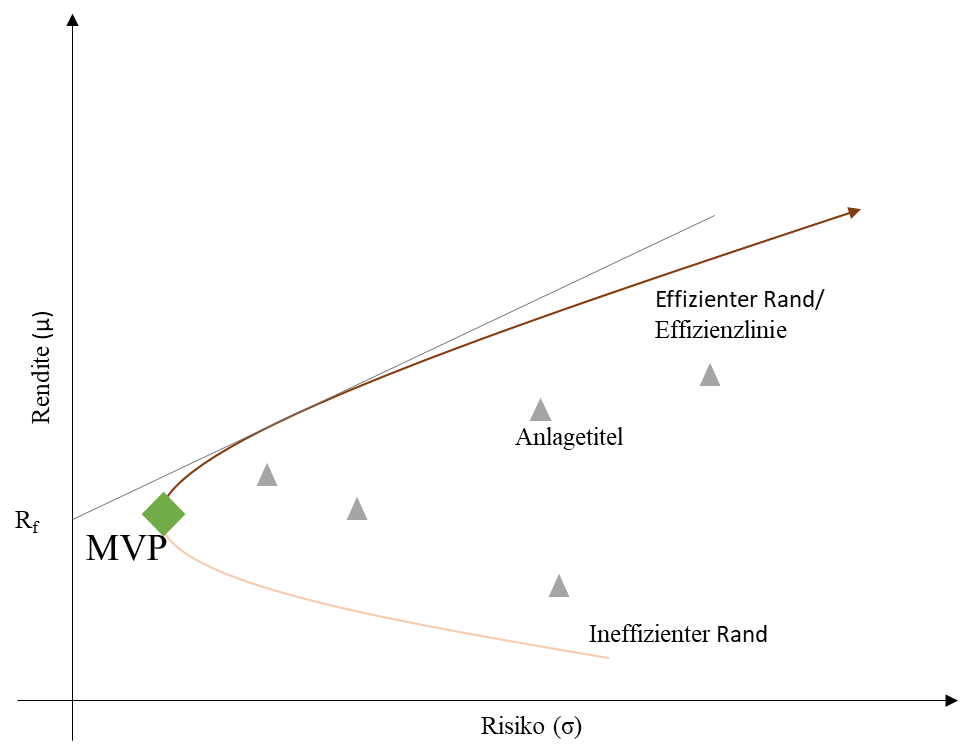
\includegraphics[width=0.8\textwidth]{Abbildungen/abb_effizienzlinie.png}
  \caption{MV-Portfolio, Effizienzlinie}
  \label{abb:effizienzlinie}
  \begin{minipage}{\linewidth}\vspace{0.4em}\centering\footnotesize
  Eigene Darstellung.
  \end{minipage}
\end{figure}

Eine wesentliche theoretische Eigenschaft des unbeschränkten MVP besteht darin, dass der marginale Risikobeitrag jedes Vermögenswerts identisch ist und der Volatilität des Gesamtportfolios entspricht.
Daraus folgt, dass der prozentuale Beitrag eines Vermögenswerts zum Gesamtrisiko seinem jeweiligen Portfoliogewicht entspricht.
Darüber hinaus ist die Kovarianz jedes einzelnen Vermögenswerts mit dem MVP gleich der Varianz des MVP, sodass das Beta sämtlicher Vermögenswerte in Bezug auf dieses Portfolio den Wert eins annimmt.
Diese Zusammenhänge gelten für die unbeschränkte Optimierung und müssen bei zusätzlichen Gewichtsbeschränkungen nicht mehr für sämtliche Vermögenswerte erfüllt sein.

Ein wesentlicher Vorteil des MVP liegt darin, dass keine erwarteten Renditen geschätzt werden müssen, deren zuverlässige Bestimmung mit erheblichen statistischen Schwierigkeiten verbunden ist (Merton, 1980)\todo{Quelle Merton (1980) fehlt in literatur/bibliography.bib}.
Dadurch kann eine zentrale Quelle von Schätzfehlern vermieden werden.
Allerdings bleibt das Verfahren empfindlich gegenüber Fehlschätzungen der Varianzen und Korrelationen.
Insbesondere bei einer unbeschränkten Optimierung können bereits geringe Veränderungen der geschätzten Kovarianzmatrix zu deutlichen Verschiebungen der Portfoliogewichte führen.
Empirische Hinweise auf die praktische Bedeutung der Minimum-Varianz-Strategie liefern \textcite{behr2008}.
Für den US-Aktienmarkt im Zeitraum von 1968 bis 2007 zeigen sie, dass Minimum-Varianz-Portfolios insbesondere in Phasen hoher Marktvolatilität und Unsicherheit positive und signifikante Renditen erzielen können.
Gegenüber einem wertgewichteten Benchmark zeigte sich eine höhere Performance, während gegenüber einem gleichgewichteten Portfolio keine statistisch signifikante Verbesserung der Sharpe Ratio festgestellt wurde.
Die Ergebnisse sprechen damit vor allem für das Potenzial des MVP zur Risikoreduzierung, nicht zwangsläufig für eine höhere risikoadjustierte Rendite.

Eine zentrale Schwäche des MVP ist die mögliche Konzentration auf wenige Vermögenswerte.
Da ausschließlich die Gesamtvarianz minimiert wird, können einzelne Positionen hohe Gewichte erhalten, während andere vollständig ausgeschlossen werden.
\textcite{lee2011} zeigt dies anhand von zehn Sektoren des Russell-1000-Universums, bei denen unter der Beschränkung auf nicht negative Gewichte vier Sektoren ein Gewicht von null erhielten.
Auch \textcite{maillard2010} weisen auf diese Konzentrationsanfälligkeit hin.
Die Portfoliozusammensetzung wird dabei nicht allein von den individuellen Volatilitäten bestimmt, sondern ebenso von den Korrelationen zwischen den Vermögenswerten.
Daher können auch Anlagen mit höherer Einzelvolatilität das Gesamtrisiko reduzieren, wenn sie günstige Diversifikationseigenschaften aufweisen.
Gewichtsbeschränkungen können einer übermäßigen Konzentration entgegenwirken und zugleich einen regulierenden Effekt auf Schätzfehler der Kovarianzmatrix haben (Jagannathan \& Ma, 2003)\todo{Quelle Jagannathan \& Ma (2003) fehlt in literatur/bibliography.bib}.

Eine weitere theoretische Besonderheit ergibt sich unter der Annahme identischer erwarteter Renditen aller Vermögenswerte.
Da in diesem Fall sämtliche vollständig investierten Portfolios dieselbe erwartete Rendite aufweisen, stellt das MVP aufgrund seines geringsten Risikos zugleich das optimale Mean-Variance-Portfolio dar.
Liegt die gemeinsame erwartete Rendite oberhalb des risikofreien Zinssatzes, entspricht es zudem dem Tangentialportfolio mit der höchsten Sharpe Ratio \parencite{lee2011,chaves2011}.

\paragraph{Gleichgewichtetes Portfolio (1/N-Portfolio)}
Das 1/N-Portfolio, auch bekannt als gleichgewichtete Portfoliostrategie, ist eine einfache Anlagestrategie, bei der jeder der $n$ risikoreichen Vermögenswerte im Portfolio mit einem gleichmäßigen Gewicht gehalten wird.
Die Formel zur Berechnung der Gewichte im 1/N-Portfolio lautet:
\begin{equation}
	w = \frac{1}{n}
	\label{eq:naiv}
\end{equation}

Hierbei repräsentiert $w$ das Gewicht des Vermögenswerts und $n$ die Gesamtanzahl der Vermögenswerte im Portfolio.
Ein wesentlicher Vorteil der 1/N-Strategie liegt in ihrer einfachen und robusten Konstruktion.
Für die Bestimmung der Portfoliogewichte müssen weder erwartete Renditen noch Varianzen oder Kovarianzen geschätzt werden.
Dadurch werden Schätzfehler vermieden, die bei optimierungsbasierten Verfahren die Portfolioallokation erheblich beeinflussen können.
Gleichzeitig wirkt die gleichmäßige Kapitalverteilung einer starken Konzentration auf einzelne Positionen entgegen.

Die praktische Bedeutung der 1/N-Strategie zeigen \textcite{demiguel2009}.
Die Autoren verglichen die Out-of-Sample-Performance von 14 optimierten Portfoliomodellen, darunter klassische Mean-Variance-Modelle, bayesianische Ansätze und Modelle mit Gewichtsbeschränkungen, anhand von sieben empirischen Datensätzen mit der Gleichgewichtung.
Keines der untersuchten Modelle konnte die 1/N-Strategie hinsichtlich Sharpe Ratio, Certainty-Equivalent Return (CEQ) und Portfolioumschlag konsistent übertreffen.
Als wesentliche Ursache identifizieren die Autoren Schätzfehler bei erwarteten Renditen und der Kovarianzmatrix, die zu ungünstigen Portfoliogewichten führen können.
Um diese ausreichend zu reduzieren, wären teilweise sehr lange historische Beobachtungszeiträume erforderlich.
Die Ergebnisse zeigen damit, dass eine höhere mathematische Komplexität nicht zwangsläufig zu einer besseren Out-of-Sample-Performance führt.

Die Befunde von \textcite{demiguel2009} werden in der nachfolgenden Literatur jedoch differenziert betrachtet.
\textcite{kritzman2010} argumentieren, dass die Ergebnisse zugunsten der 1/N-Strategie unter anderem von kurzen historischen Schätzfenstern beeinflusst werden können und optimierte Portfolios bei langfristigeren Renditeannahmen bessere Ergebnisse erzielen können.
\textcite{kirby2012} zeigen ebenfalls, dass die relative Performance von der Modellgestaltung abhängt.
Geeignete Zielrenditen sowie alternative Gewichtungsansätze auf Grundlage von Volatilitäts- oder Rendite-Risiko-Signalen können der Gleichgewichtung auch unter Berücksichtigung von Transaktionskosten überlegen sein.
\textcite{tu2011} verfolgen einen kombinierten Ansatz, bei dem die 1/N-Strategie mit optimierten Portfolios verbunden wird, um die Robustheit der Gleichgewichtung mit den Vorteilen einer risikoorientierten Optimierung zu vereinen.

Trotz ihrer Robustheit weist die 1/N-Strategie Einschränkungen hinsichtlich der Risikodiversifizierung auf.
Da unterschiedliche Volatilitäten und Korrelationen bei der Gewichtung nicht berücksichtigt werden, können besonders volatile Vermögenswerte einen überproportionalen Anteil am Gesamtrisiko ausmachen.
Dies kann insbesondere in turbulenten Marktphasen relevant sein.
Risikoorientierte Verfahren wie das Minimum-Varianz-Portfolio berücksichtigen diese Risikostruktur gezielt und können dadurch Vorteile bei der Begrenzung des Portfoliorisikos bieten \parencite[vgl.][S.~165]{savona2019}.

\paragraph{Das Equal-Risk-Contribution-Portfolio}
Das Equal-Risk-Contribution-Portfolio (ERC) stellt einen risikobasierten Ansatz zur Portfoliooptimierung dar, dessen Grundlagen unter anderem von Qian (2005)\todo{Quelle Qian (2005) fehlt in literatur/bibliography.bib} und Neukirch (2008)\todo{Quelle Neukirch (2008) fehlt in literatur/bibliography.bib} entwickelt und von \textcite{maillard2010} näher untersucht wurden.
Im Gegensatz zum gleichgewichteten Portfolio (1/N), bei dem das Kapital gleichmäßig auf sämtliche Vermögenswerte verteilt wird, und zum Minimum-Varianz-Portfolio (MVP), das die Gesamtvarianz minimiert, strebt ERC eine gleichmäßige Verteilung der Risikobeiträge an.
Die Portfoliogewichte werden so bestimmt, dass jeder Vermögenswert unabhängig von seinem Kapitalanteil den gleichen Beitrag zum Gesamtrisiko leistet.
Dabei werden sowohl die individuellen Volatilitäten als auch die Korrelationen zwischen den Vermögenswerten berücksichtigt.

Grundlage der ERC-Portfoliokonstruktion ist der Risikobeitrag eines Vermögenswerts, der sich aus seinem Portfoliogewicht und seinem marginalen Risikobeitrag (Marginal Risk Contribution, MRC) ergibt.
Der MRC beschreibt, wie sich das Gesamtrisiko des Portfolios verändert, wenn das Gewicht eines Vermögenswerts geringfügig erhöht wird.
Die Portfoliogewichte werden anschließend so gewählt, dass die daraus resultierenden Risikobeiträge aller Vermögenswerte übereinstimmen.
\begin{equation}
	\mathrm{MRC}_i = \frac{\partial \sigma(w)}{\partial w_i} = \frac{(V w)_i}{\sigma(w)}
	\label{eq:erc-mrc}
\end{equation}

Dabei steht $\sigma(w)$ für die Standardabweichung des Portfolios, $V$ für die Varianz-Kovarianz-Matrix und $w$ für den Vektor der Portfoliogewichte.
Die Portfoliovolatilität wird dann als Summe der absoluten Risikobeiträge (ARC) aller Vermögenswerte berechnet.
Jeder ARC gibt an, wie viel Risiko ein Vermögenswert zum Gesamtrisiko des Portfolios beiträgt, und ermöglicht somit eine detaillierte Analyse der einzelnen Risikokomponenten im Portfolio:
\begin{equation}
	\sigma(w) = \sum_{i=1}^{n} \mathrm{ARC}_i
	\label{eq:erc-arc}
\end{equation}

Hierbei ist $\mathrm{ARC}_i = w_i \cdot \mathrm{MRC}_i$ der absolute Risikobeitrag des Vermögenswerts $i$.
Um sicherzustellen, dass alle Vermögenswerte im Portfolio einen gleichmäßigen Beitrag zum Risiko leisten, wird die Differenz zwischen den absoluten Risikobeiträgen jedes Vermögenswerts minimiert.
Dies geschieht durch die Lösung eines Optimierungsproblems, bei dem das Ziel ist, die Quadratsumme der Differenzen zwischen den ARC-Werten aller Vermögenswerte zu minimieren:
\begin{equation}
	\min_{w} f(w), \qquad \text{wobei} \quad f(w) = \sum_{i=1}^{n}\sum_{j=1}^{n}\left(\mathrm{ARC}_i - \mathrm{ARC}_j\right)^2
	\label{eq:erc-ziel}
\end{equation}

Dabei ist $f(w)$ die Zielfunktion, die die Quadratsumme der Differenzen zwischen den ARC-Werten aller Vermögenswerte im Portfolio darstellt.
Anders als das MVP nutzt ERC die Kovarianzmatrix somit nur über das Produkt $V w$ und nicht über ihre Inverse, weshalb Schätzfehler weniger stark durchschlagen.

\textcite{maillard2010} beschreiben ERC als einen Ansatz, der Eigenschaften des gleichgewichteten Portfolios und des Minimum-Varianz-Portfolios miteinander verbindet.
Während das MVP zu einer starken Konzentration auf einzelne Vermögenswerte führen kann, werden bei ERC unter den üblichen Annahmen einer positiv definiten Kovarianzmatrix und nicht negativer Gewichte sämtliche Vermögenswerte berücksichtigt.
Die Gesamtvarianz des ERC-Portfolios ist jedoch mindestens so hoch wie die des MVP, da die gleichmäßige Risikoverteilung nicht auf eine Minimierung des Gesamtrisikos ausgerichtet ist.
\textcite{lee2011} zeigt zudem, dass Vermögenswerte mit niedriger Volatilität häufig höhere Kapitalgewichte erhalten, um die Risikobeiträge der einzelnen Positionen anzugleichen.

Empirische Untersuchungen liefern unterschiedliche Ergebnisse zur Leistungsfähigkeit der ERC-Strategie.
\textcite{chaves2011} vergleichen verschiedene Allokationsverfahren anhand eines breit diversifizierten Anlageuniversums aus Anleihen, Aktien, Rohstoffen und Immobilien.
ERC erzielte dabei nicht durchgehend bessere Ergebnisse als das 1/N-Portfolio, zeigte jedoch gegenüber dem MVP und klassischen Mean-Variance-Portfolios in den untersuchten Konstellationen günstigere Ergebnisse.
Gleichzeitig verdeutlichen die Autoren, dass die Performance risikobasierter Strategien von der Zusammensetzung des Anlageuniversums abhängt.
Insbesondere eine hohe Gewichtung von Anleihen kann deren historische Performance in Phasen sinkender Zinsen begünstigen.

\textcite{savona2019} vergleichen ERC anhand von Daten aus dem Zeitraum von 2001 bis 2013 mit Markowitz-, Minimum-Varianz- und gleichgewichteten Portfolios.
Ergänzende Monte-Carlo- und Bootstrap-Analysen dienten der Überprüfung der Robustheit der Ergebnisse.
Die dynamische ERC-Strategie erzielte gegenüber einzelnen Vergleichsstrategien, insbesondere dem MVP und dem 1/N-Portfolio, statistisch signifikante Überrenditen.
Das Tangentialportfolio wies jedoch in mehreren Konstellationen eine höhere Performance und Diversifizierung auf.
Auch \textcite{bastin2018} findet für den deutschen Aktienmarkt von 2002 bis 2015 günstige Ergebnisse.
Im untersuchten CDAX-Anlageuniversum erreichte ERC mit 0,32 die höchste Sharpe Ratio der betrachteten Strategien, eine gegenüber dem Gesamtmarkt um etwa 50\,\% geringere Volatilität sowie ein statistisch signifikantes positives CAPM-Alpha von 7,5\,\% pro Jahr.

Die relative Leistungsfähigkeit von ERC kann zudem von der jeweiligen Marktphase abhängen.
\textcite{escobar2013} zeigen, dass während turbulenter Marktphasen risikoorientierte Verfahren wie ERC und MVP gegenüber der 1/N-Strategie Vorteile hinsichtlich der risikoadjustierten Performance aufweisen können.
Zudem kann eine Anpassung der Portfolioallokation an unterschiedliche Marktregime höhere Sharpe Ratios ermöglichen als eine ausschließlich statische Gewichtungsstrategie.

Neben der Performance ist die Robustheit gegenüber Schätzfehlern von Bedeutung.
\textcite{ardia2017} untersuchen die Sensitivität risikobasierter Strategien gegenüber Fehlspezifikationen der Kovarianzmatrix.
ERC und die Inverse-Volatility-Methode erwiesen sich dabei als vergleichsweise robust, während das MVP stärker auf Schätzfehler reagierte.
Allerdings ist auch ERC von der Qualität der Risikoschätzungen abhängig, wobei Fehler in den individuellen Varianzen die Portfoliozusammensetzung stärker beeinflussen können als Fehler in den Korrelationen.
Insgesamt bietet ERC einen Mittelweg zwischen der einfachen Gleichgewichtung und der konsequenten Varianzminimierung des MVP.
Durch die Gleichverteilung der Risikobeiträge wird eine stärkere Risikodiversifizierung angestrebt, ohne erwartete Renditen schätzen zu müssen.
Die empirischen Ergebnisse zeigen jedoch, dass die Performance von den Marktbedingungen, dem Anlageuniversum und der Qualität der geschätzten Risikoparameter abhängt.

\paragraph{Die Hierarchical Risk Parity}
Der Hierarchical-Risk-Parity-Algorithmus (HRP) wurde von \textcite{deprado2016} als alternativer Ansatz zur Portfolioallokation entwickelt.
Er kombiniert Methoden der Graphentheorie mit hierarchischen Clustering-Verfahren des unüberwachten maschinellen Lernens.
Ziel ist es, Schwächen klassischer Portfoliooptimierungsverfahren zu reduzieren.
Insbesondere die Mean-Variance-Optimierung kann aufgrund von Schätzfehlern in den erwarteten Renditen und der Kovarianzmatrix zu instabilen Portfoliogewichten und einer hohen Konzentration auf einzelne Vermögenswerte führen.
HRP berücksichtigt die Abhängigkeitsstrukturen zwischen den Vermögenswerten, ohne dass eine Invertierung der Kovarianzmatrix erforderlich ist.
Dadurch kann das Verfahren auch bei schlecht konditionierten oder singulären Kovarianzmatrizen eingesetzt werden.

Die Konstruktion des HRP-Portfolios erfolgt in drei aufeinanderfolgenden Schritten: hierarchisches Clustering, Quasi-Diagonalisierung und hierarchische Zweiteilung.
Im ersten Schritt werden die Vermögenswerte anhand ihrer Ähnlichkeiten hierarchisch gruppiert.
Als Grundlage dient ein Distanzmaß, das üblicherweise aus den Pearson-Korrelationskoeffizienten der Vermögenswertrenditen abgeleitet wird.
Dadurch entsteht eine hierarchische Baumstruktur, das sogenannte Dendrogramm (siehe \hyperref[abb:dendrogramm]{Abbildung~\ref*{abb:dendrogramm}}), in der Vermögenswerte mit ähnlichen Renditeverläufen zu Clustern zusammengefasst werden.
Anschließend wird die Kovarianzmatrix im Rahmen der Quasi-Diagonalisierung entsprechend der ermittelten Clusterstruktur umgeordnet.
Eng miteinander verbundene Vermögenswerte werden dadurch innerhalb der Matrix nebeneinander angeordnet und die Abhängigkeitsstruktur wird sichtbar gemacht.
Im abschließenden Schritt, der hierarchischen Zweiteilung, wird das verfügbare Kapital schrittweise entlang der Baumstruktur verteilt.
Die Cluster werden auf jeder Ebene in zwei Teilgruppen aufgeteilt, deren Kapitalanteile anhand ihrer jeweiligen Varianzen bestimmt werden.
Cluster mit höherer Varianz erhalten einen geringeren Kapitalanteil, während risikoärmere Cluster stärker gewichtet werden.
Auf diese Weise berücksichtigt HRP sowohl die Risikoeigenschaften der Vermögenswerte als auch deren Abhängigkeitsstruktur.

\begin{figure}[htbp]
  \centering
  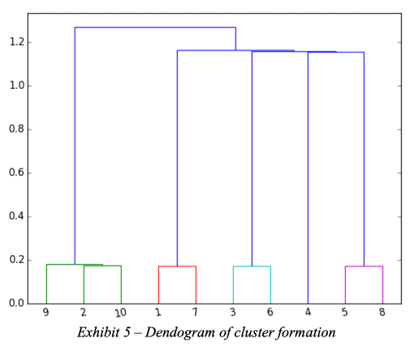
\includegraphics[width=0.65\textwidth]{Abbildungen/abb_dendrogramm.png}
  \caption{Dendrogramm der Clusterbildung}
  \label{abb:dendrogramm}
  \begin{minipage}{\linewidth}\vspace{0.4em}\centering\footnotesize
  Entnommen aus \textcite{deprado2016}.
  \end{minipage}
\end{figure}

\textcite{deprado2016} untersuchte die Leistungsfähigkeit des HRP-Algorithmus anhand von Out-of-Sample-Monte-Carlo-Simulationen mit 10.000 Durchläufen und unterschiedlichen Marktschocks.
Als Vergleich dienten ein mit dem Critical Line Algorithm (CLA) konstruiertes Minimum-Varianz-Portfolio sowie ein nach inverser Volatilität gewichtetes Portfolio (IVP).
HRP wies in den Simulationen eine geringere Out-of-Sample-Varianz auf und erzielte gegenüber dem CLA eine um etwa 31,3\,\% höhere Sharpe Ratio.
Während der CLA aufgrund hoher Positionskonzentrationen insbesondere gegenüber idiosynkratischen Schocks anfällig war und das IVP die Korrelationsstruktur nicht unmittelbar berücksichtigte, zeigte sich HRP durch die Einbeziehung der Clusterstruktur gegenüber den untersuchten Schocks vergleichsweise robust.

Weitere empirische Erkenntnisse liefert \textcite{sen2022}, der HRP mit dem CLA am indischen Aktienmarkt verglich.
Die Untersuchung umfasste den Nifty~50 sowie acht Branchensektoren mit einem Trainingszeitraum von 2016 bis 2020 und einem Out-of-Sample-Test im Jahr 2021.
HRP erzielte in sieben der acht untersuchten Sektoren eine höhere Sharpe Ratio und führte zu einer ausgewogeneren Verteilung der Kapitalgewichte.
Der CLA wies dagegen teilweise eine stärkere Konzentration auf einzelne Vermögenswerte auf.

Neben der Performance stellt der Portfolioumschlag eine praktische Herausforderung des HRP-Ansatzes dar.
Untersuchungen von \textcite{lohre2020} zeigen, dass Veränderungen der geschätzten Clusterstruktur bei einer auf Pearson-Korrelationen basierenden HRP-Strategie zu häufigeren Portfolioanpassungen führen können.
In den untersuchten Backtests lag der jährliche Portfolioumschlag bei etwa 18\,\% bis 23\,\%, während traditionelle Risk-Parity-Portfolios Werte zwischen 3,5\,\% und 5\,\% erreichten.
Die daraus entstehenden Transaktionskosten können die Nettoperformance von HRP reduzieren.

Darüber hinaus wurden Erweiterungen entwickelt, um extreme Marktrisiken stärker zu berücksichtigen.
Ein Ansatz verwendet den Lower Tail Dependence Coefficient (LTDC) als alternatives Distanzmaß.
Während die Pearson-Korrelation vor allem lineare Zusammenhänge zwischen Renditen erfasst, berücksichtigt der LTDC die gemeinsame Abhängigkeit der Vermögenswerte bei extrem negativen Renditeentwicklungen.
Dadurch kann die Clusterbildung stärker am gemeinsamen Verlustverhalten ausgerichtet werden.
In Bootstrap-Simulationen wiesen LTDC-basierte HRP-Portfolios geringere Maximum Drawdowns sowie eine stabilere Clusterstruktur und moderatere Umschlagshäufigkeit als die auf Pearson-Korrelationen basierende Variante auf.

Insgesamt stellt HRP einen risikobasierten Allokationsansatz dar, der Abhängigkeitsstrukturen zwischen Vermögenswerten durch hierarchisches Clustering unmittelbar in die Portfoliokonstruktion einbezieht und ohne Invertierung der Kovarianzmatrix auskommt.
Empirische Untersuchungen weisen auf mögliche Vorteile hinsichtlich Risikodiversifizierung, Gewichtungsstabilität und risikoadjustierter Performance hin.
Die tatsächliche Leistungsfähigkeit hängt jedoch von der Qualität der Risikoschätzungen, dem verwendeten Distanzmaß und der Stabilität der Clusterstruktur ab.
Veränderungen der Abhängigkeitsstrukturen können zudem häufigere Portfolioanpassungen und damit höhere Transaktionskosten verursachen.

% =============================================================================
\section{Bewertungskriterien}\label{sec:kriterien}

\subsection{Statistische Verlustmaße}
Die Prognosequalität wird über zwei Verlustmaße gemessen, den multivariaten Quasi-Likelihood-Verlust (QLIKE), oder auch Stein-Loss genannt \parencite{laurent2013}, und den Mean Squared Error (MSE) der Kovarianzmatrix.
Da die wahre bedingte Kovarianzmatrix der Testperiode nicht beobachtbar ist, wird die Prognose bei beiden gegen denselben realisierten Proxy gemessen.
\begin{align}
	\label{eq:proxy}
	S &= \frac{1}{h}\sum_{t=1}^{h} r_t\,r_t' \\
	\label{eq:qlike}
	\mathrm{QLIKE}(\Sigma, S) &= \ln|\Sigma| + \operatorname{tr}(\Sigma^{-1} S) \\
	\label{eq:mse}
	\mathrm{MSE}(\Sigma, S) &= \frac{1}{N^2}\sum_{i,j}\left(\Sigma_{ij} - S_{ij}\right)^2
\end{align}

Dabei ist $\Sigma$ die prognostizierte und $S$ die realisierte Kovarianzmatrix, $r_t$ der Vektor der logarithmierten Tagesrenditen und $N$ die Anzahl der zur Verfügung stehenden Sektorindizes im jeweiligen Zeitfenster.
Beide Verluste werden je Rebalancierungsfenster berechnet und anschließend über die Fenster gemittelt, wobei niedrigere Werte eine bessere Prognose bedeuten.

Die beiden Maße unterscheiden sich darin, wie sie Fehler in beide Richtungen gewichten.
Der QLIKE-Verlust aus \hyperref[eq:qlike]{Gleichung~\ref*{eq:qlike}} bestraft eine Unterschätzung des Risikos stärker als eine Überschätzung, während der MSE aus \hyperref[eq:mse]{Gleichung~\ref*{eq:mse}} Über- und Unterschätzungen gleichgewichtet.
Aus ökonomischer Sicht wiegt eine Unterschätzung des Risikos schwerer als eine Überschätzung, weshalb die Asymmetrie des QLIKE-Verlusts hier erwünscht ist.

Diese beiden Maße werden verwendet, da sie sich in anderen Studien als robust gegenüber verrauschten Proxys erwiesen haben.
Dies ist insbesondere relevant, da der Proxy für $h=1$ allein aus dem äußeren Produkt eines einzigen Renditevektors besteht und somit stark verrauscht ist.
So konnten \textcite{patton2011} und \textcite{laurent2013} zeigen, dass beide Metriken Kovarianzmatrizen unabhängig von der Genauigkeit des Proxys robust ordnen.
Folglich ist der absolute Wert der Metriken zwar nur eingeschränkt interpretierbar, jedoch ist die Rangfolge robust, weshalb Qualitätsunterschiede zwischen den Schätzern erkannt werden können.
Da zusätzlich die Länge des Trainingsfensters die Zahl der investierbaren Anlagen und damit die Dimension der Kovarianzmatrix beeinflusst, sind Vergleiche zwischen den unterschiedlichen Trainingsfenstern ebenfalls mit Vorsicht zu interpretieren.
Aussagekräftig ist daher in erster Linie die Differenz zwischen den Schätzern innerhalb einer Spezifikation.

Da der QLIKE-Verlust ökonomisch besser motiviert ist, wird dieser als primäre Vergleichsmetrik verwendet, während der MSE als weitere Metrik zur Überprüfung der Robustheit dient.

\subsection{Ökonomische Kennzahlen}
Als ökonomische Kennzahlen werden die annualisierte Rendite, die realisierte Volatilität, die Sharpe Ratio und der Turnover berichtet.
Die folgenden Kennzahlen beruhen auf der Tagesrendite der verschiedenen Portfolios $r_{p,t}$.
\begin{align}
	\label{eq:annrendite}
	R_{\mathrm{ann}} &= \left(\prod_{t=1}^{n}\left(1 + r_{p,t}\right)\right)^{\frac{252}{n}} - 1 \\
	\label{eq:annvola}
	\sigma_{\mathrm{ann}} &= \sqrt{252}\;\operatorname{sd}\left(r_{p,t}\right) \\
	\label{eq:sharpe}
	\text{Sharpe Ratio} &=\frac{252\;\overline{\left(r_{p,t} - r_{f,t}\right)}}{\sqrt{252}\;\operatorname{sd}\left(r_{p,t} - r_{f,t}\right)}
\end{align}

Die annualisierte Rendite aus \hyperref[eq:annrendite]{Gleichung~\ref*{eq:annrendite}} ist die geometrische Wachstumsrate über die $n$ Handelstage des Bewertungszeitraums, während die realisierte Volatilität als annualisierte Standardabweichung derselben Reihe berechnet wird.
Bei der Sharpe Ratio beruhen Zähler und Nenner auf der Überschussrendite gegenüber der Fed Funds Rate.

Neben diesen Metriken wird auch der Turnover beachtet, der angibt, welcher Anteil des Portfolios je Rebalancierung umgeschichtet wird.
\begin{equation}
	\mathrm{Turnover}_k = \sum_{i=1}^{N}\left| w_{i,k}^{\mathrm{Ziel}} - w_{i,k-1}^{\mathrm{Ende}} \right|
	\label{eq:turnover}
\end{equation}

Dabei sind $w_{i,k}^{\mathrm{Ziel}}$ die neuen Zielgewichte der Rebalancierung $k$ und $w_{i,k-1}^{\mathrm{Ende}}$ die über die vorangegangene Halteperiode gedrifteten Endgewichte.
Der Turnover dient dabei als Proxy für Transaktionskosten und zugleich als Indiz für die Robustheit der Optimierungsverfahren.
In dieser Studie werden die Transaktionskosten bei der Rebalancierung zwar nicht direkt berücksichtigt, jedoch werden die Auswirkungen kurz bei den Ergebnissen und in \hyperref[sec:anhang_kosten]{Anhang~\ref*{sec:anhang_kosten}} dargestellt.

\subsection{Signifikanztests}
Signifikanzaussagen beruhen auf zwei Tests.
Unterschiede in der Prognosegüte werden mit dem Diebold-Mariano-Test (DM-Test) auf die Verlustdifferenzen geprüft \parencite{diebold1995,west1996}, deren Langfristvarianz autokorrelationsrobust geschätzt wird.
Für Unterschiede in den Sharpe Ratios dient der Test von \textcite{jobson1981} in der Korrektur von \textcite{memmel2003}, der die Korrelation der beiden Renditereihen berücksichtigt.
Damit wird für beide Bewertungsebenen getrennt geprüft, ob die beobachteten Unterschiede zwischen den Schätz- und Optimierungsverfahren über zufällige Schwankungen hinausgehen.

% =============================================================================
\section{Ergebnisse und Diskussion}\label{sec:ergebnisse}
Zunächst wird geprüft, ob die GARCH-basierten Schätzer die Kovarianzmatrix besser prognostizieren, bevor untersucht wird, ob sich ein solcher Vorteil auch in der Portfolioperformance niederschlägt.
Diese Reihenfolge folgt dem Einwand von \textcite{engle2006}, wonach die Sharpe Ratio von den realisierten Renditen dominiert wird, auf die die Kovarianzmatrix nur mittelbar wirkt, was sich ebenso auf andere renditebasierte Kennzahlen übertragen lässt.
Anschließend wird die Stabilität beider Befunde über Trainingsfenster und Prognosehorizonte betrachtet, während der Einfluss des Bewertungszeitraums und der Teilperioden im \hyperref[sec:anhang_strukturbruch]{Anhang~\ref*{sec:anhang_strukturbruch}} behandelt wird.

% -----------------------------------------------------------------------------
\subsection{Statistische Prognosequalität}\label{sec:statistisch}
Im Basisfall (vier Jahre Training, ein Tag Prognosehorizont) ordnet sich die Prognosegüte unter beiden Verlustmaßen nach der Modellkomplexität, wie \hyperref[tab:statistik_basis]{Tabelle~\ref*{tab:statistik_basis}} zeigt.
Die historische Matrix schneidet am schlechtesten ab, während der GARCH-Schätzer sie deutlich verbessert und DCC-GARCH nochmals einen kleinen Zusatzgewinn liefert.
QLIKE und MSE stimmen hierbei in dieser Reihenfolge überein.

% automatisch erzeugt von paper/tabellen.py -- nicht von Hand editieren
\begin{table}[htbp]
  \centering
  \footnotesize
  \begin{tabular}{lrr}
    \toprule
    Kovarianzschätzer & QLIKE & MSE ($\times 10^{-7}$) \\
    \midrule
    Historisch & -152,81 & 4,28 \\
    GARCH & -155,37 & 3,52 \\
    DCC-GARCH & -156,12 & 3,44 \\
    \bottomrule
  \end{tabular}
  \caption{Prognosequalität der Kovarianzschätzer im Basisfall}
  \label{tab:statistik_basis}
  \begin{minipage}{\linewidth}\vspace{0.4em}\centering\footnotesize
  TRBC, Training 1008 Handelstage, Prognosehorizont 1 Tag, bewertet über die volle Historie vom 12.02.2003 bis 09.06.2026; niedrigere Werte bedeuten eine bessere Prognose. QLIKE gemittelt über 6013 Termine, an denen alle drei Schätzer definiert sind (die historische Matrix ist an einzelnen Terminen singulär); MSE über alle 6079 Termine, an denen dieser Ausfall nicht auftritt.
  \end{minipage}
\end{table}


Wie scharf die beiden Verlustmaße trennen, unterscheidet sich allerdings erheblich.
Der DM-Test in \hyperref[tab:dmw]{Tabelle~\ref*{tab:dmw}} verwirft die Nullhypothese gleicher erwarteter Verluste unter QLIKE in allen drei paarweisen Vergleichen auf dem 1-\%-Niveau, wobei dies trotz der insgesamt geringen Differenz auch für den Vergleich von DCC-GARCH und GARCH gilt.
Der Grund hierfür liegt darin, dass beide Schätzer dieselben Varianzprognosen verwenden, wodurch die Verlustdifferenz kaum streut und fast ausschließlich aus dem Korrelationsbeitrag stammt.
Unter dem MSE sind die Abstände zur historischen Matrix hingegen nur auf dem 5-\%-Niveau signifikant, während der Unterschied zwischen DCC und GARCH nicht mehr von null zu trennen ist.
Belastbar ist somit, dass beide dynamischen Schätzer die historische Matrix unter dem primären QLIKE-Kriterium hochsignifikant schlagen und auch der Zusatznutzen der dynamischen Korrelation dort nachweisbar ist, während der MSE nur die gröbere Rangfolge bestätigt.

% automatisch erzeugt von paper/tabellen.py -- nicht von Hand editieren
\begin{table}[htbp]
  \centering
  \footnotesize
  \begin{tabular}{lrrr@{}lr}
    \toprule
    Vergleich & $\varnothing\,\Delta$ Verlust & $t$-Statistik & \multicolumn{2}{c}{$p$-Wert} & Termine \\
    \midrule
    \multicolumn{6}{l}{\textit{QLIKE}} \\
    \quad GARCH vs.\ Historisch & -2,563 & -4,18 & $<$0,001 & $^{***}$ & 6013 \\
    \quad DCC-GARCH vs.\ Historisch & -3,308 & -5,28 & $<$0,001 & $^{***}$ & 6013 \\
    \quad DCC-GARCH vs.\ GARCH & -0,744 & -13,86 & $<$0,001 & $^{***}$ & 6079 \\
    \midrule
    \multicolumn{6}{l}{\textit{MSE ($\times 10^{-7}$)}} \\
    \quad GARCH vs.\ Historisch & -0,764 & -2,23 & 0,026 & $^{**}$ & 6079 \\
    \quad DCC-GARCH vs.\ Historisch & -0,846 & -2,11 & 0,035 & $^{**}$ & 6079 \\
    \quad DCC-GARCH vs.\ GARCH & -0,082 & -1,26 & 0,207 &  & 6079 \\
    \bottomrule
  \end{tabular}
  \caption{Diebold-Mariano-Tests auf die Verlustdifferenzen (Basisfall)}
  \label{tab:dmw}
  \begin{minipage}{\linewidth}\vspace{0.4em}\centering\footnotesize
  Basisfall, bewertet über die volle Historie vom 12.02.2003 bis 09.06.2026. Negative Differenzen bedeuten, dass der erstgenannte Schätzer besser prognostiziert; $^{***}$, $^{**}$, $^{*}$ = 1-, 5-, 10-\%-Niveau.
  \end{minipage}
\end{table}


Über das gesamte Untersuchungsdesign hinweg ist der statistische Vorsprung nahezu vollständig, da DCC-GARCH unter dem primären QLIKE-Kriterium in 37 von 40~Kombinationen und unter dem MSE in sämtlichen 40 besser prognostiziert als die historische Matrix (siehe \hyperref[tab:bestzaehlung]{Tabelle~\ref*{tab:bestzaehlung}} im Anhang).
Da alle Läufe für diesen Vergleich denselben Bewertungszeitraum ab 2010 nutzen und sich ihre Trainingsfenster stark überlappen, ist diese Auszählung als Robustheit über Spezifikationen hinweg und nicht als 40 voneinander unabhängige Bestätigungen zu verstehen.
Wie stark der Vorsprung ausfällt, hängt jedoch von der Spezifikation ab, wie \hyperref[tab:qlike_grid]{Tabelle~\ref*{tab:qlike_grid}} zeigt.
Mit der Länge des Trainingsfensters nimmt er bis etwa fünf Jahren zu und stabilisiert sich danach, wobei bei einjährigem Training unter QLIKE kein Vorteil vorliegt und der GARCH-Schätzer sogar schlechter abschneidet als die historische Matrix.
Eine mögliche Erklärung hierfür ist, dass die dynamischen Modelle insgesamt mehr Parameter schätzen müssen und deshalb bei einer geringen Datenbasis schlechter abschneiden, obwohl ihre Annahmen näher an der Realität liegen.
Beim MSE ist die Ordnung nach Modellkomplexität dagegen über alle dargestellten Trainingsfenster und Prognosehorizonte hinweg vorzufinden.

Über den Prognosehorizont bleibt der Vorsprung unter QLIKE dagegen nahezu konstant, während er unter dem MSE relativ zum Verlustniveau sogar zunimmt.
Wie jedoch im \hyperref[sec:kriterien]{Abschnitt zu den Bewertungskriterien} dargelegt, verändert sich mit der Fensterlänge wegen der später beginnenden Zeitreihen auch die Zahl der investierbaren Sektoren, weshalb die Entwicklung über die Trainingsfenster nur mit Vorsicht interpretiert werden sollte.

% automatisch erzeugt von paper/tabellen.py -- nicht von Hand editieren
\begin{table}[htbp]
  \centering
  \footnotesize
  \begin{tabular}{lrrrrrr}
    \toprule
    & \multicolumn{3}{c}{QLIKE} & \multicolumn{3}{c}{MSE ($\times 10^{-7}$)} \\
    \cmidrule(lr){2-4}\cmidrule(lr){5-7}
    Spezifikation & Historisch & GARCH & DCC-GARCH & Historisch & GARCH & DCC-GARCH \\
    \midrule
    252 & -176,1 & -175,9 & -176,1 & 2,99 & 2,48 & 2,47 \\
    504 & -171,0 & -171,4 & -171,8 & 3,42 & 2,81 & 2,74 \\
    756 & -165,2 & -166,1 & -166,8 & 3,41 & 2,84 & 2,75 \\
    1008 & -159,7 & -161,1 & -161,9 & 3,43 & 2,87 & 2,77 \\
    1260 & -154,3 & -156,1 & -157,1 & 3,42 & 2,83 & 2,75 \\
    1512 & -150,1 & -151,8 & -152,9 & 3,18 & 2,60 & 2,52 \\
    1764 & -146,0 & -147,7 & -148,8 & 3,11 & 2,53 & 2,45 \\
    2016 & -142,0 & -143,8 & -144,9 & 3,09 & 2,52 & 2,45 \\
    2268 & -140,6 & -142,5 & -143,7 & 3,05 & 2,46 & 2,41 \\
    2520 & -140,0 & -142,0 & -143,3 & 3,02 & 2,45 & 2,40 \\
    \midrule
    $h=1$ & -159,7 & -161,1 & -161,9 & 3,43 & 2,87 & 2,77 \\
    $h=5$ & -159,5 & -160,9 & -161,6 & 1,68 & 1,23 & 1,17 \\
    $h=10$ & -159,3 & -160,9 & -161,5 & 1,32 & 0,95 & 0,90 \\
    $h=21$ & -158,9 & -160,2 & -160,7 & 0,82 & 0,49 & 0,46 \\
    \bottomrule
  \end{tabular}
  \caption{Prognosequalität über Trainingsfenster und Prognosehorizonte (TRBC)}
  \label{tab:qlike_grid}
  \begin{minipage}{\linewidth}\vspace{0.4em}\centering\footnotesize
  Beide Blöcke bewertet ab 01.01.2010. Oberer Block: Trainingsfenster in Handelstagen bei $h=1$, unterer Block: Prognosehorizonte bei 1008 Tagen Training.
  \end{minipage}
\end{table}


Neben der bereits genannten Dimensionsabhängigkeit des QLIKE ist im unteren Block zu beachten, dass der Proxy über $h$ Tage mittelt und damit umso weniger streut, je länger der Horizont ist.
Das MSE-Niveau fällt deshalb über die Horizonte, ohne dass die Prognosen dort besser wären, während dies beim QLIKE-Verlust nicht zu beobachten ist.
Für die zweite Forschungsfrage fällt die statistische Antwort dennoch eindeutig aus, da beide dynamischen Modelle die Prognose der Kovarianzmatrix im Basisfall signifikant verbessern und DCC-GARCH die historische Schätzung unter QLIKE in nahezu allen und unter dem MSE in sämtlichen 40~Kombinationen schlägt.

% -----------------------------------------------------------------------------
\subsection{Ökonomische Performance}\label{sec:oekonomisch}
Die ökonomische Auswertung führt zu einem differenzierteren Bild.
Für die erste Forschungsfrage zeigt \hyperref[tab:oekonomie_basis]{Tabelle~\ref*{tab:oekonomie_basis}} zunächst, dass alle neun risikobasierten Kombinationen im Basisfall eine höhere Sharpe Ratio erreichen als das naive 1/N-Portfolio, bei ERC mit dynamischer Kovarianz allerdings nur um wenige Tausendstel.
Vorne liegt dabei das MVP, gefolgt von HRP und ERC.
Der Vorsprung entsteht vollständig auf der Risikoseite, da das 1/N-Portfolio zwar die höchste Rendite im Feld erzielt, diese aber mit der mit Abstand höchsten Volatilität erkauft.

% automatisch erzeugt von paper/tabellen.py -- nicht von Hand editieren
\begin{table}[htbp]
  \centering
  \footnotesize
  \begin{tabular}{llrrrrr}
    \toprule
    Modell & Kovarianz & Rendite (\%) & Vola (\%) & Sharpe & Turnover & Anlagen $>1\,\%$ \\
    \midrule
    MVP & Historisch & 9,03 & 13,82 & 0,567 & 0,008 & 4,6 \\
    MVP & GARCH & 8,55 & 13,94 & 0,532 & 0,258 & 4,9 \\
    MVP & DCC-GARCH & 8,65 & 13,81 & 0,543 & 0,255 & 4,9 \\
    \midrule
    HRP & Historisch & 9,27 & 16,74 & 0,509 & 0,012 & 17,6 \\
    HRP & GARCH & 8,96 & 16,21 & 0,502 & 0,072 & 17,4 \\
    HRP & DCC-GARCH & 9,13 & 16,17 & 0,513 & 0,094 & 17,4 \\
    \midrule
    ERC & Historisch & 9,46 & 17,67 & 0,501 & 0,006 & 17,8 \\
    ERC & GARCH & 9,14 & 17,32 & 0,490 & 0,034 & 17,8 \\
    ERC & DCC-GARCH & 9,13 & 17,31 & 0,490 & 0,034 & 17,8 \\
    \midrule
    1/N & -- & 9,58 & 18,79 & 0,488 & 0,006 & 17,8 \\
    \bottomrule
  \end{tabular}
  \caption{Out-of-Sample-Performance im Basisfall}
  \label{tab:oekonomie_basis}
  \begin{minipage}{\linewidth}\vspace{0.4em}\centering\footnotesize
  TRBC, Training 1008 Handelstage, Prognosehorizont 1 Tag, bewertet über die volle Historie vom 12.02.2003 bis 09.06.2026; Rendite, Volatilität und Sharpe Ratio annualisiert, Turnover ohne Kosten; Anlagen $>1\,\%$ ist die durchschnittliche Zahl der Sektoren mit einem Gewicht von mehr als 1\,\% je Formationstermin.
  \end{minipage}
\end{table}


%% automatisch erzeugt von paper/abbildungen.py -- nicht von Hand editieren
\begin{figure}[htbp]
  \centering
  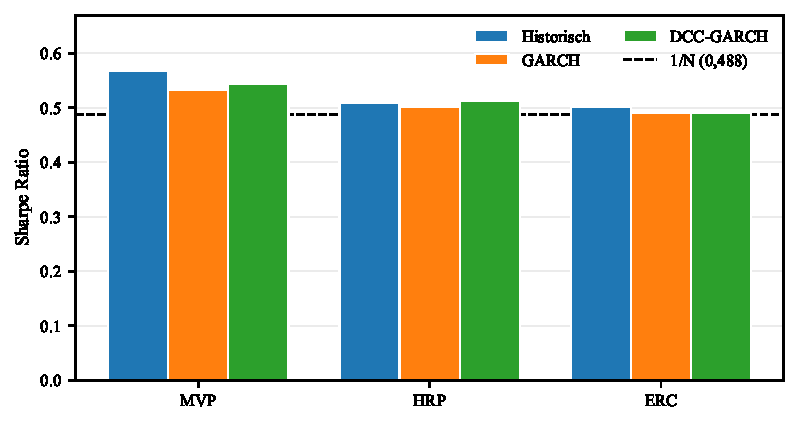
\includegraphics[width=0.88\textwidth]{Abbildungen/abb_sharpe_basis.pdf}
  \caption{Sharpe Ratio der Portfoliomodelle im Basisfall}
  \label{abb:sharpe_basis}
  \begin{minipage}{\linewidth}\vspace{0.4em}\centering\footnotesize
  TRBC, Training 1008 Handelstage, Prognosehorizont 1 Tag; die gestrichelte Linie markiert das 1/N-Portfolio.
  \end{minipage}
\end{figure}


Innerhalb der Portfoliomodelle kehrt sich die statistische Rangfolge im Basisfall weitgehend um, da bei MVP und ERC die historische Matrix vorne liegt und allein beim HRP der DCC-Schätzer marginal besser abschneidet.
Der GARCH-Schätzer bleibt dabei in allen drei Modellen hinter der historischen Matrix zurück.
Bei HRP und ERC senken die dynamischen Schätzer jedoch die realisierte Volatilität spürbar, während der DCC-Schätzer beim MVP auf einem ähnlichen Niveau wie der historische Schätzer liegt, wobei dieser Vorteil in der Sharpe Ratio durch die Einbindung der Rendite jeweils verschwindet.
Genau diese Größe schlagen \textcite{engle2006} für das Minimum-Varianz-Portfolio als ökonomisches Auswahlkriterium vor, da dessen realisierte Volatilität unmittelbar von der Kovarianzmatrix abhängt und nicht von den Renditen überlagert wird.
Diese Idee kann auch auf HRP und ERC übertragen werden, da deren Gewichte ebenfalls allein aus der Kovarianzmatrix stammen.

Gleichzeitig fällt der mittlere Turnover des MVP mit der DCC- wie auch mit der GARCH-Kovarianz rund 32-mal so hoch aus wie mit der historischen, wodurch beide dynamischen Schätzer bei einer realen Umsetzung nochmals schlechter abschneiden würden.
Grund für den hohen Turnover ist, dass die beiden dynamischen Modelle deutlich schneller auf Änderungen in der Volatilität reagieren, wodurch auch die Gewichtsverteilung der Portfolios angepasst wird, während die träge Stichprobenkovarianz die Gewichte nahezu unverändert lässt.
Bei HRP und ERC fällt der Anstieg mit dem Faktor 5 bis 8 erheblich geringer aus, was auf die robustere Konstruktion der beiden Modelle zurückzuführen ist.

Wie unterschiedlich die Verfahren das Kapital verteilen, zeigt die durchschnittliche Zahl der Sektoren mit einem Gewicht von mehr als 1\,\% in \hyperref[tab:oekonomie_basis]{Tabelle~\ref*{tab:oekonomie_basis}}. Das MVP konzentriert sich im Mittel auf nur vier bis fünf der rund 18 investierbaren Sektoren, während HRP und ERC nahezu alle Sektoren nennenswert gewichten. Diese deutlich breitere Streuung trägt letztlich zur höheren Robustheit von HRP und ERC bei.

Statistisch abgesichert sind die Unterschiede in der Sharpe Ratio allerdings nicht, da \hyperref[tab:jobson_korkie]{Tabelle~\ref*{tab:jobson_korkie}} im \hyperref[sec:anhang_sharpetests]{Anhang~\ref*{sec:anhang_sharpetests}} für keinen der relevanten Vergleiche einen auch nur annähernd signifikanten $p$-Wert ausweist.
Dies gilt sowohl zwischen den Kovarianzschätzern als auch gegenüber dem 1/N-Portfolio.

Die Auswirkungen proportionaler Transaktionskosten sind in \hyperref[tab:transaktionskosten]{Tabelle~\ref*{tab:transaktionskosten}} im \hyperref[sec:anhang_kosten]{Anhang~\ref*{sec:anhang_kosten}} dargestellt.
Bereits bei 5~Basispunkten auf das umgeschlagene Volumen fällt die Sharpe Ratio des MVP mit DCC-Kovarianz von 0,543 auf 0,310 und liegt damit deutlich unter dem naiven Portfolio mit 0,484, während die historische Variante mit 0,560 nahezu unverändert bleibt.
Bei 20~Basispunkten werden beide dynamischen MVP-Varianten negativ.

\hyperref[tab:bilanz]{Tabelle~\ref*{tab:bilanz}} fasst die Ergebnisse über alle 40~Kombinationen aus Trainingsfenster und Prognosehorizont zusammen, wobei je Portfoliomodell angegeben wird, wie oft das 1/N-Portfolio geschlagen wird und wie oft die dynamischen Schätzer die historische Matrix übertreffen.
Bewertungsmaßstab ist dabei die Sharpe Ratio, wobei der Befund je nach Portfoliomodell unterschiedlich ausfällt.
Zur ersten Forschungsfrage zeigt sich, dass HRP und ERC mit historischer Kovarianz das 1/N-Portfolio in rund 90 Prozent der Konstellationen schlagen, das MVP dagegen nur in einem Fünftel der Fälle.
Ausschlaggebend ist die bereits angelegte Anfälligkeit des MVP, dass Schätzfehler im Optimierungsprozess verstärkt werden, wodurch konzentrierte Portfolios entstehen.
Die im Basisfall beste Sharpe Ratio des MVP ist insofern nicht repräsentativ.

Zur zweiten Forschungsfrage zeigt sich ein klares Muster entlang der Portfoliomodelle, da die dynamischen Schätzer die historische Matrix beim MVP in mehr als der Hälfte der Läufe schlagen, beim HRP nur vereinzelt und beim ERC in keinem einzigen.
Ökonomisch ist das gut erklärbar, weil das MVP als einziges Verfahren die Kovarianzmatrix vollständig einschließlich ihrer Inversen ausnutzt, während HRP lediglich die Clusterordnung und die Varianzen der Teilcluster verwendet und ERC die Risikobeiträge ausbalanciert.
Eine bessere Kovarianzprognose zahlt sich folglich dort aus, wo sie am intensivsten genutzt wird, und bleibt folgenlos, wo das Verfahren die Matrix nur grob verwendet.
Somit steht das ökonomische Ergebnis im Gegensatz zum statistischen Befund.

% automatisch erzeugt von paper/tabellen.py -- nicht von Hand editieren
\begin{table}[htbp]
  \centering
  \footnotesize
  \begin{tabular}{llrr}
    \toprule
    Modell & Kovarianz & vs.\ 1/N & vs.\ historischer Matrix \\
    \midrule
    MVP & Historisch & 8/40 & -- \\
    MVP & GARCH & 15/40 & 22/40 \\
    MVP & DCC-GARCH & 17/40 & 26/40 \\
    \midrule
    HRP & Historisch & 35/40 & -- \\
    HRP & GARCH & 16/40 & 2/40 \\
    HRP & DCC-GARCH & 19/40 & 3/40 \\
    \midrule
    ERC & Historisch & 36/40 & -- \\
    ERC & GARCH & 17/40 & 0/40 \\
    ERC & DCC-GARCH & 20/40 & 0/40 \\
    \bottomrule
  \end{tabular}
  \caption{Ergebnisse über alle empirischen Läufe}
  \label{tab:bilanz}
  \begin{minipage}{\linewidth}\vspace{0.4em}\centering\footnotesize
  Alle 40 Kombinationen aus Trainingsfenster und Prognosehorizont, bewertet ab 01.01.2010; ausgewiesen ist, wie oft die Sharpe Ratio höher ausfällt als beim jeweiligen Vergleichsmaßstab.
  \end{minipage}
\end{table}


Auch über die Trainingsfenster hinweg bleibt dieses Muster erhalten (\hyperref[abb:sharpe_train]{siehe Abb.~\ref*{abb:sharpe_train}}).
Beim MVP liegt DCC in allen zehn Fenstern über der historischen Matrix, bei HRP in einem und bei ERC in keinem.
Der GARCH-Schätzer folgt diesem Muster bei HRP und ERC, erreicht beim MVP mit sechs von zehn Fenstern aber einen deutlich schwächeren Vorsprung als DCC.
Dass DCC hier beim MVP vorne liegt, während im Basisfall die historische Matrix führt, ist kein Widerspruch, sondern ein Zeitraumeffekt, da diese Vergleiche auf dem gemeinsamen Zeitraum ab 2010 beruhen und das MVP mit dynamischer Kovarianz gerade in der Phase 2010--2019 vorne liegt (\hyperref[sec:anhang_strukturbruch]{siehe Anhang~\ref*{sec:anhang_strukturbruch}}).
Die absoluten Unterschiede fallen dabei klein aus, weshalb angesichts der insignifikanten Tests auf Sharpe-Differenzen keine belastbare Rangfolge abgeleitet werden sollte.

%% automatisch erzeugt von paper/tabellen.py -- nicht von Hand editieren
\begin{table}[htbp]
  \centering
  \footnotesize
  \begin{tabular}{rrrrrrrrrrr}
    \toprule
    Training & \multicolumn{3}{c}{MVP} & \multicolumn{3}{c}{HRP} & \multicolumn{3}{c}{ERC} & 1/N \\
    \cmidrule(lr){2-4}\cmidrule(lr){5-7}\cmidrule(lr){8-10}
     & Hist. & GARCH & DCC & Hist. & GARCH & DCC & Hist. & GARCH & DCC & \\
    \midrule
    252 & 0,515 & 0,505 & 0,518 & 0,600 & 0,580 & 0,568 & 0,595 & 0,585 & 0,583 & 0,592 \\
    504 & 0,495 & 0,627 & 0,633 & 0,602 & 0,605 & 0,595 & 0,599 & 0,592 & 0,591 & 0,601 \\
    756 & 0,525 & 0,561 & 0,564 & 0,603 & 0,589 & 0,590 & 0,600 & 0,588 & 0,588 & 0,593 \\
    1008 & 0,606 & 0,599 & 0,620 & 0,592 & 0,592 & 0,611 & 0,604 & 0,591 & 0,592 & 0,594 \\
    1260 & 0,613 & 0,592 & 0,620 & 0,594 & 0,575 & 0,578 & 0,587 & 0,574 & 0,576 & 0,573 \\
    1512 & 0,574 & 0,562 & 0,587 & 0,593 & 0,573 & 0,574 & 0,587 & 0,573 & 0,576 & 0,576 \\
    1764 & 0,535 & 0,563 & 0,578 & 0,564 & 0,547 & 0,554 & 0,554 & 0,545 & 0,546 & 0,537 \\
    2016 & 0,525 & 0,545 & 0,547 & 0,565 & 0,555 & 0,553 & 0,562 & 0,555 & 0,556 & 0,545 \\
    2268 & 0,550 & 0,581 & 0,574 & 0,579 & 0,560 & 0,562 & 0,573 & 0,565 & 0,565 & 0,551 \\
    2520 & 0,521 & 0,582 & 0,580 & 0,587 & 0,569 & 0,566 & 0,581 & 0,572 & 0,572 & 0,563 \\
    \bottomrule
  \end{tabular}
  \caption{Sharpe Ratios über die Trainingsfenster (TRBC, $h=1$)}
  \label{tab:sharpe_train}
  \begin{minipage}{\linewidth}\vspace{0.4em}\centering\footnotesize
  Annualisierte Sharpe Ratio, bewertet ab 01.01.2010.
  \end{minipage}
\end{table}


% automatisch erzeugt von paper/abbildungen.py -- nicht von Hand editieren
\begin{figure}[htbp]
  \centering
  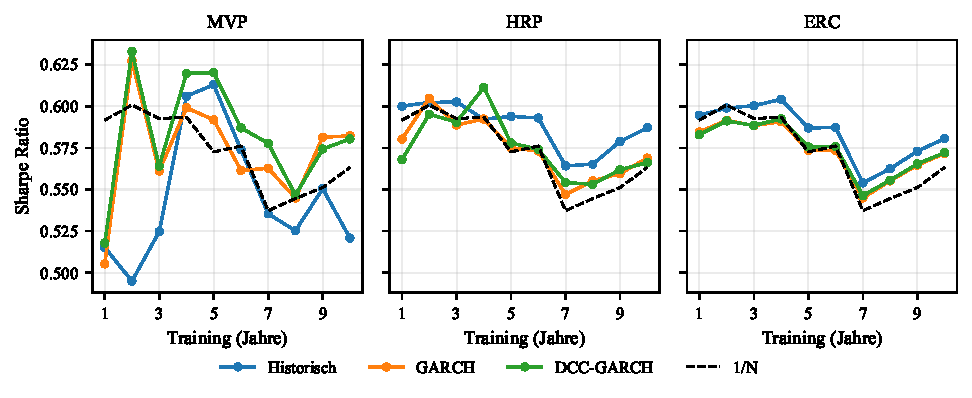
\includegraphics[width=\textwidth]{Abbildungen/abb_sharpe_train.pdf}
  \caption{Sharpe Ratio über die Trainingsfenster}
  \label{abb:sharpe_train}
  \begin{minipage}{\linewidth}\vspace{0.4em}\centering\footnotesize
  TRBC, Prognosehorizont 1 Tag, Bewertung ab 01.01.2010 für alle Fenster.
  \end{minipage}
\end{figure}


Deutlicher ist der Befund über den Prognosehorizont in \hyperref[tab:sharpe_horizont]{Tabelle~\ref*{tab:sharpe_horizont}}.
Der tägliche Basisfall dient dabei vor allem dazu, den Effekt der Kovarianzdynamik ohne die Nebenwirkungen seltenerer Rebalancierung zu isolieren, jedoch werden in der Realität auch längere Rebalancierungszyklen relevant.
Wird seltener rebalanciert, bleibt die Sharpe Ratio der historischen Matrix beim MVP praktisch konstant, während sie für DCC und ebenso für GARCH bei den beiden längeren Horizonten deutlich fällt und der Turnover je Rebalancierung gleichzeitig auf mehr als das Doppelte steigt.
Der Verlauf ist dabei nicht monoton, da beide dynamischen Schätzer bei einem Horizont von fünf Tagen zunächst ihren höchsten Wert im gesamten Feld erreichen und erst danach zurückfallen.
Eine Erklärung hierfür ist, dass sich die historisch geschätzte Kovarianzmatrix nur langsam mit der Zeit verändert, weshalb ihre Prognose schon bei kurzen Vorhersagezeiträumen keine aktuelle Dynamik abbildet und über eine längere Halteperiode entsprechend wenig veraltet.
Die GARCH-Modelle hingegen reflektieren Abweichungen nahezu sofort, weshalb ihre Prognose zwar den Formationszeitpunkt genau trifft, über die Halteperiode hinweg aber schnell veraltet.
Das Maximum bei fünf Tagen deutet darauf hin, dass ein Teil der täglichen Umschichtungen auf Schätzrauschen und nicht auf verwertbare Dynamik reagiert, sodass dessen Wegfall die Performance zunächst verbessert, bevor das Veralten der Prognose überwiegt.
Erkennbar ist das auch am Turnover, da dessen hohes Niveau anzeigt, wie stark sich die Kovarianzmatrix der dynamischen Modelle über eine längere Halteperiode verändert.
Aufgrund der selteneren Rebalancierung fällt der über die gesamte Historie kumulierte Turnover trotz des höheren Werts je Rebalancierung jedoch geringer aus, womit auch die Kostenbelastung einer realen Umsetzung sinken würde.
Bei HRP und ERC bleiben die Sharpe Ratios hingegen weitestgehend stabil, was wiederum auf die Robustheit dieser Verfahren hindeutet.

% automatisch erzeugt von paper/tabellen.py -- nicht von Hand editieren
\begin{table}[htbp]
  \centering
  \footnotesize
  \begin{tabular}{rrlrrrr}
    \toprule
    $h$ (Tage) & 1/N & Kovarianz & MVP & HRP & ERC & Turnover MVP \\
    \midrule
    1 & 0,594 & Historisch & 0,606 & 0,592 & 0,604 & 0,008 \\
     &  & GARCH & 0,599 & 0,592 & 0,591 & 0,258 \\
     &  & DCC-GARCH & 0,620 & 0,611 & 0,592 & 0,255 \\
    \midrule
    5 & 0,597 & Historisch & 0,597 & 0,588 & 0,605 & 0,021 \\
     &  & GARCH & 0,639 & 0,587 & 0,592 & 0,527 \\
     &  & DCC-GARCH & 0,654 & 0,596 & 0,594 & 0,522 \\
    \midrule
    10 & 0,601 & Historisch & 0,610 & 0,600 & 0,610 & 0,033 \\
     &  & GARCH & 0,524 & 0,578 & 0,589 & 0,603 \\
     &  & DCC-GARCH & 0,545 & 0,575 & 0,590 & 0,598 \\
    \midrule
    21 & 0,602 & Historisch & 0,615 & 0,605 & 0,612 & 0,058 \\
     &  & GARCH & 0,524 & 0,598 & 0,598 & 0,587 \\
     &  & DCC-GARCH & 0,532 & 0,595 & 0,600 & 0,587 \\
    \bottomrule
  \end{tabular}
  \caption{Sharpe Ratios und Turnover über die Prognosehorizonte (TRBC, Training 1008 Tage)}
  \label{tab:sharpe_horizont}
  \begin{minipage}{\linewidth}\vspace{0.4em}\centering\footnotesize
  Annualisierte Sharpe Ratio, bewertet ab 01.01.2010; Turnover je Rebalancierung, also nicht auf gleiche Frequenz normiert.
  \end{minipage}
\end{table}


% -----------------------------------------------------------------------------
\subsection{Einordnung in die Literatur}\label{sec:literatur}
Die berichteten Befunde lassen sich abschließend gegen die eingangs skizzierte Literatur halten.

Dass alle drei risikobasierten Verfahren das naive Portfolio im Basisfall übertreffen, widerspricht zunächst \textcite{demiguel2009}.
Deren Argument greift hier jedoch nur zur Hälfte, da von den beiden Schätzfehlerquellen allein die Kovarianzmatrix verbleibt.
Nach \textcite{broadie1993} richten gerade die erwarteten Renditen den größeren Schaden an.
Hinzu kommt das Anlageuniversum, denn breit diversifizierte Sektorindizes lassen sich stabiler schätzen als Einzeltitel.

Die Unterschiede zwischen den Verfahren fügen sich dagegen gut in die vorliegende Evidenz ein.
HRP schlägt das naive Portfolio in 35 von 40 Läufen und stützt damit die Robustheit, die \textcite{deprado2016} und \textcite{sen2022} berichten, auch wenn dort gegen ein varianzminimierendes statt gegen ein gleichgewichtetes Portfolio verglichen wird.
Für ERC gilt die Einschränkung von \textcite{chaves2011}, da der Vorsprung gegenüber dem naiven Portfolio im Basisfall nur wenige Tausendstel beträgt.
Deutlich ausgeprägter ist dagegen ihr zweiter Befund, dass ERC das Minimum-Varianz-Portfolio übertrifft, denn ERC liegt in 36 von 40 Läufen über dem naiven Portfolio und das MVP nur in acht.
Hinter dieser Schwäche des MVP steht die Fehlermaximierung, die \textcite{michaud1989} beschreibt, sichtbar in der von \textcite{lee2011} dokumentierten Konzentration auf wenige Anlagen.
Am genauesten entspricht das Bild jedoch \textcite{behr2008}, denn dort wie hier senkt das MVP das Risiko spürbar, ohne die Sharpe Ratio gegenüber dem gleichgewichteten Portfolio signifikant zu verbessern.

Für die zweite Forschungsfrage ist der Abstand zwischen statistischem und ökonomischem Ergebnis der entscheidende Punkt.
Dass die Tests auf Sharpe-Differenzen durchweg insignifikant ausfallen, bestätigt den Einwand von \textcite{engle2006} für den vorliegenden Datensatz.
Die robusten Verlustfunktionen von \textcite{patton2011} und \textcite{laurent2013} trennen auf denselben Daten dagegen klar.
Beide Kriterien verhalten sich damit genau so, wie es die jeweiligen Arbeiten erwarten lassen.
Auch \textcite{ardia2017} stehen nur scheinbar im Widerspruch, denn eine verzerrte Kovarianzmatrix wird erst dort teuer, wo ein Verfahren sie intensiv nutzt.
Ihre Einordnung, nach der das MVP empfindlicher reagiert als ERC, bildet sich hier ab, denn ein Schätzerwechsel bewegt Sharpe Ratio und Turnover des MVP um ein Mehrfaches stärker.
Robustheit hat damit ihren Preis, da ein Verfahren, das eine schlechte Schätzung verzeiht, aus einer besseren auch keinen Nutzen zieht.
Die größte Nähe besteht zu \textcite{moura2020}, die für hochdimensionale Kovarianzmatrizen ebenfalls finden, dass die statistisch beste Spezifikation nicht die ökonomisch beste sein muss.
Dieser bereits existente ökonomische Nachteil würde durch Transaktionskosten noch verstärkt werden.

Jedes der beiden Ergebnisse ist für sich in der Literatur belegt, ihre Verbindung dagegen kaum, da Arbeiten zur Kombination risikobasierter Allokation mit multivariaten GARCH-Prognosen bislang selten sind.

% =============================================================================
\section{Limitationen}\label{sec:limitationen}
Die Aussagekraft der Ergebnisse ist in mehrfacher Hinsicht begrenzt, wobei die Einschränkungen im Folgenden nach ihrem Gewicht für die Interpretation geordnet werden.

Eine zentrale Limitation ist dabei, dass der Backtest ohne Handelskosten rechnet und Kosten nur nachträglich als proportionaler Abschlag berücksichtigt werden, obwohl sich die Verfahren im Turnover um den Faktor~32 unterscheiden.
Die berichteten Kennzahlen begünstigen damit die dynamischen Schätzer, deren Nachteil unter realen Kosten größer ausfiele als ausgewiesen.
Umgekehrt wird die Aussage des \hyperref[sec:oekonomisch]{Abschnitts zur ökonomischen Performance} dadurch nicht geschwächt, sondern verschärft, da dieser Nachteil bereits ohne Kosten vorhanden ist.

Auf der Messseite ist der realisierte Proxy die wesentliche Einschränkung, da er für $h = 1$ aus einem einzigen äußeren Produkt besteht und damit den Rang eins hat.
Beide Verlustfunktionen bleiben nach \textcite{patton2011} und \textcite{laurent2013} unabhängig von der Genauigkeit des Proxys rangerhaltend, jedoch begrenzt das geringe Signal-Rausch-Verhältnis die Teststärke des DM-Tests, wobei der MSE stärker betroffen ist als der QLIKE-Verlust.
Intraday-Daten würden einen erheblich präziseren Proxy liefern, standen für diese Arbeit aber nicht zur Verfügung.
Hinzu kommt, dass ausschließlich die relative Prognosegüte bewertet wurde und nicht die absolute Kalibrierung der prognostizierten Volatilität.
Ob die Modelle das Risikoniveau im Mittel treffen, bleibt damit offen.

Des Weiteren beruht die gesamte Auswertung auf einem einzigen Universum, dessen Sektorindizes rechnerische Größen sind und sich nicht unmittelbar handeln lassen, weshalb eine direkte Replikation der optimierten Portfolios nicht möglich ist.
Gezeigt ist damit, dass die Befunde für diese Datengrundlage gelten, nicht aber, ob sie sich auf andere Märkte übertragen lassen.

% [Vorschlag 2.1] Limitation zu 260 vs. 252 Handelstagen/Jahr auf Wunsch
% wieder entfernt, siehe Kommentar in Abschnitt 2.1.
%\neu{Auf der Datenseite enthalten die Sektorreihen Feiertage als Handelstage mit Nullrendite, da Datastream sie mit dem Kurs des Vortages auffüllt (\hyperref[sec:daten]{Abschnitt~\ref*{sec:daten}}).

\subsection{Ausblick}\label{sec:forschung}
Aus den Ergebnissen und den genannten Einschränkungen ergeben sich vier Ansatzpunkte für weitere Untersuchungen.

Auf der Modellseite wird ausschließlich ein GARCH(1,1) geschätzt, obwohl dieses Modell im Vergleich zur Realität vereinfachte Annahmen trifft.
Beispielsweise zeigt sich in empirischen Untersuchungen, dass negative Schocks in der Regel einen stärkeren Einfluss auf die nachfolgende Volatilität haben als positive.
Anders als das einfache GARCH-Modell binden Modelle wie GJR-GARCH und EGARCH diese Asymmetrie ein und sind somit realitätsnäher, während sich über höhere Ordnungen oder ein GARCH-MIDAS zusätzlich längerfristige Komponenten der Volatilität erfassen lassen.
Da der ökonomische Nachteil der dynamischen Schätzer hier hauptsächlich aus dem Turnover und nicht aus der Prognosegüte stammt, wäre allerdings zu prüfen, ob eine realitätsnähere Varianzdynamik daran überhaupt etwas ändert.

Auf der Allokationsseite ließe sich das Feld um modernere Verfahren wie Hierarchical Equal Risk Contribution \parencite{raffinot2018herc} oder Nested Clustered Optimization \parencite{deprado2019nco} erweitern, die die hierarchische Struktur von HRP anders auswerten.
Beide nutzen die Kovarianzmatrix intensiver als HRP, ohne sie wie das MVP vollständig zu invertieren.
Da sich der Mehrwert einer besseren Prognose in dieser Arbeit genau danach richtet, wie intensiv ein Verfahren die Matrix nutzt, ließe sich an ihnen prüfen, ob der Zusammenhang auch auf den Stufen dazwischen gilt.
Offen bleibt zudem, ob eine bessere Kovarianzmatrix in Verfahren, die zusätzlich eine Renditeprognose verwenden, einen größeren Vorteil liefert, da die Matrix dort nicht nur das Risiko begrenzt, sondern auch die Gewichtung der erwarteten Renditen bestimmt.

Der dritte Ansatzpunkt betrifft die Transaktionskosten, die hier weder im Backtest noch in der Optimierung berücksichtigt werden.
Ein kostenbewusster Optimierer würde den Turnover in die Zielfunktion aufnehmen und dadurch einen Teil der Belastung vermeiden, statt sie nur zu erleiden.
Ob die dynamischen Schätzer unter einer solchen Nebenbedingung weiterhin zurückfallen, ist offen und wäre für die praktische Bewertung der entscheidende Test.

Schließlich sollten die Befunde an weiteren Datensätzen überprüft werden, etwa an Einzeltiteln, anderen Regionen oder Anlageklassen mit geringerer durchschnittlicher Korrelation.
Gerade die hohe paarweise Korrelation des hier verwendeten Universums begrenzt die Diversifikationsmöglichkeiten von vornherein und könnte den Spielraum für eine bessere Kovarianzprognose systematisch verengen.

% =============================================================================
\section{Fazit}\label{sec:fazit}
Die Arbeit hat zwei Fragen getrennt untersucht, nämlich ob risikobasierte Portfoliomodelle das naive 1/N-Portfolio schlagen und ob GARCH-basierte Kovarianzprognosen gegenüber der historischen Schätzung einen Mehrwert stiften.

Zur ersten Frage hängt die Antwort stark vom gewählten Verfahren ab.
HRP und ERC mit historischer Kovarianz übertreffen das 1/N-Portfolio in rund neun von zehn untersuchten Konstellationen und erweisen sich als robust gegenüber Variationen von Trainings- und Prognosefenster.
Das Minimum-Varianz-Portfolio erzielt im Basisfall zwar die höchste Sharpe Ratio, schlägt 1/N über alle Läufe hinweg aber nur in einem Fünftel der Fälle und reagiert am empfindlichsten auf Schätzfehler.
Für die Praxis sprechen diese Ergebnisse damit eher für die robusteren Verfahren als für die Varianzminimierung, wobei einschränkend gilt, dass keiner der Vorsprünge gegenüber 1/N statistisch signifikant ist.

Zur zweiten Frage entscheidet das angelegte Kriterium über die Antwort, worin zugleich der Hauptbefund liegt.
Statistisch ist das Ergebnis eindeutig, da DCC-GARCH die Kovarianzmatrix in allen 40~Läufen unter dem MSE und in nahezu allen unter dem QLIKE-Verlust besser prognostiziert als die historische Schätzung und die Abstände zur historischen Matrix im DM-Test signifikant sind.
Ökonomisch schlägt sich dieser Vorsprung jedoch nur dort nieder, wo die Kovarianzmatrix tatsächlich intensiv genutzt wird, also beim MVP und nicht bei HRP oder ERC.
Das ist konsistent mit der Konstruktion der Verfahren, da beide die Matrix nur grob nutzen und gerade deshalb robust, zugleich aber auch unempfindlich gegenüber ihrer Verbesserung sind.
Der Preis der Dynamik ist der Turnover, der beim MVP um den Faktor~32 höher liegt und den ohnehin geringen Vorsprung unter realen Handelskosten aufzehren würde.

Der übergreifende Schluss lautet damit, dass eine bessere Risikoprognose nicht automatisch eine bessere Anlageentscheidung ist.
Die GARCH-Modelle leisten das, wofür sie konstruiert sind, und die synthetische Validierung zeigt, dass sie genau dann einen Mehrwert liefern, wenn der datengenerierende Prozess ihre Annahmen erfüllt.
Selbst dann ist dieser Mehrwert jedoch nicht garantiert.
Im DCC-Datensatz aus \hyperref[sec:anhang_synth]{Anhang~\ref*{sec:anhang_synth}} liefert das korrekt spezifizierte DCC-Modell zwar in allen zehn Trainingsfenstern den besseren QLIKE-Verlust und die niedrigere realisierte Volatilität, unterliegt beim MVP-Sharpe aber in drei von zehn Fenstern dem falsch spezifizierten GARCH-Modell.
Prognosegüte und Anlageerfolg fallen somit bereits bei bekanntem datengenerierendem Prozess auseinander.
Auf realen Sektordaten ist die verwertbare Struktur jedoch zu schwach, um die Kosten der laufenden Umschichtung zu rechtfertigen.
Nicht die Prognosegüte ist folglich die bindende Restriktion, sondern der Handel, den ihre Nutzung auslöst.


%%%%%%%%%%%%%%%%%%%%%%%%%%%%
%%%%%Ende des Dokuments%%%%%
%%%%%%%%%%%%%%%%%%%%%%%%%%%%
\newpage
\newpage


\setlength\bibitemsep{0.5\baselineskip}
\renewcommand*{\bibfont}{\setstretch{1}\normalfont\small} %kleineres Font, einfacher Zeilenabstand
\printbibliography[heading=bibintoc]
\newpage
%Nicht anfassen, so ist der Dokumentenaufbau
\addtocontents{toc}{\protect\setcounter{tocdepth}{16}}

\addappheadtotoc

\MSonehalfspacing
\appendices
\appendixpage
\appendixtitleoff
%%%%%%%%%%%%%%%%%%%%%%%%%%%%%
%%%Ab hier Inhalt einfügen%%%
%%%%%%%%%%%%%%%%%%%%%%%%%%%%%

\section{Voller und gemeinsamer Bewertungszeitraum}\label{sec:anhang_strukturbruch}
Sämtliche im Ergebnisteil berichteten Vergleiche über Trainingsfenster hinweg wurden auf dem gemeinsamen Zeitraum ab 2010 gerechnet.
Dieser Anhang begründet, warum diese Einschränkung nötig ist, und zeigt, was ohne sie gemessen würde.

Ohne die Einschränkung bewertet jedes Trainingsfenster einen anderen Zeitraum, da der Out-of-Sample-Beginn von März~2000 beim kürzesten auf November~2008 beim längsten Fenster wandert.
Der Lauf mit einem Jahr Training enthält damit das Platzen der Dotcom-Blase, während der Lauf mit zehn Jahren Training erst nach der Finanzkrise beginnt und nur die Erholung abdeckt, wodurch dessen Kennzahlen angehoben werden, ohne dass dies etwas über die Schätzqualität aussagt.
Wie stark der Effekt wiegt, zeigt \hyperref[abb:sharpe_zeitraum]{Abbildung~\ref*{abb:sharpe_zeitraum}}, in der die Sharpe Ratio über die Trainingsfenster einmal über die volle Historie und einmal über den gemeinsamen Zeitraum aufgetragen ist.
Der Sprung beim längsten Fenster tritt links auch beim 1/N-Portfolio auf, obwohl dieses überhaupt keine Schätzung vornimmt, und verschwindet rechts vollständig.
Es handelt sich somit um einen reinen Stichprobeneffekt.

% automatisch erzeugt von paper/abbildungen.py -- nicht von Hand editieren
\begin{figure}[htbp]
  \centering
  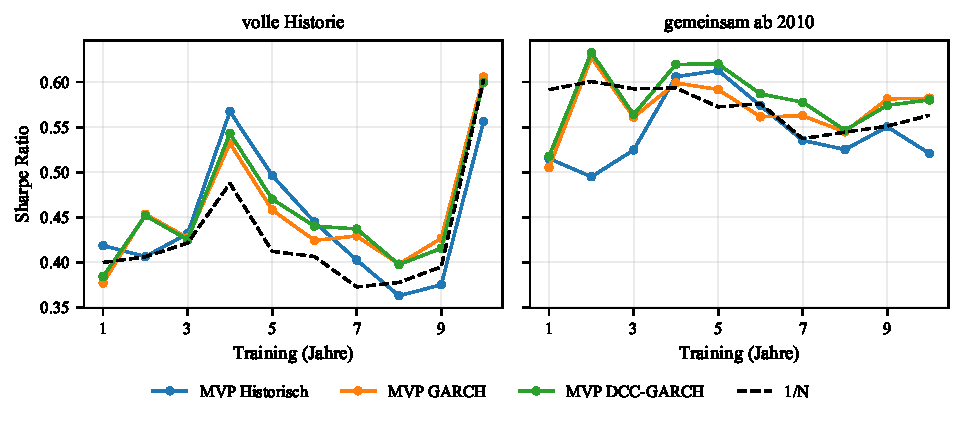
\includegraphics[width=\textwidth]{Abbildungen/abb_sharpe_zeitraum.pdf}
  \caption{Sharpe Ratio über die Trainingsfenster, voller und gemeinsamer Bewertungszeitraum}
  \label{abb:sharpe_zeitraum}
  \begin{minipage}{\linewidth}\vspace{0.4em}\centering\footnotesize
  TRBC, Prognosehorizont 1 Tag, links die volle Historie des jeweiligen Fensters, rechts der für alle Fenster identische Zeitraum ab 01.01.2010.
  \end{minipage}
\end{figure}


\hyperref[tab:strukturbruch_qlike]{Tabelle~\ref*{tab:strukturbruch_qlike}} und \hyperref[tab:strukturbruch_sharpe]{Tabelle~\ref*{tab:strukturbruch_sharpe}} stellen je Trainingsfenster die Kennzahlen über die volle Historie denen über den gemeinsamen Zeitraum ab 2010 gegenüber.
Die erste Tabelle weist neben der mittleren Größe des Anlageuniversums den QLIKE-Verlust der historischen Matrix und der beiden dynamischen Kovarianzschätzer aus, die zweite die Sharpe Ratio des MVP mit allen drei Kovarianzschätzern sowie die des 1/N-Portfolios.
Die 90-\%-Verfügbarkeitsregel lässt die zuletzt hinzugekommenen Sektoren in langen Fenstern erst spät oder gar nicht zu, weshalb die Fensterlänge über die Dimension der Kovarianzmatrix auch das QLIKE-Niveau mitbestimmt.

% automatisch erzeugt von paper/tabellen.py -- nicht von Hand editieren
\begin{table}[htbp]
  \centering
  \footnotesize
  \resizebox{\ifdim\width>\linewidth \linewidth\else \width\fi}{!}{%
  \begin{tabular}{rrrrrrrr}
    \toprule
    Training & $\varnothing\,N$ & \multicolumn{2}{c}{Historisch} & \multicolumn{2}{c}{GARCH} & \multicolumn{2}{c}{DCC-GARCH} \\
    \cmidrule(lr){3-4}\cmidrule(lr){5-6}\cmidrule(lr){7-8}
     & & voll & gem. & voll & gem. & voll & gem. \\
    \midrule
    252 & 20,3 & -161,5 & -176,1 & -161,8 & -175,9 & -162,0 & -176,1 \\
    504 & 19,7 & -159,2 & -171,0 & -160,4 & -171,4 & -160,8 & -171,8 \\
    756 & 19,1 & -156,0 & -165,2 & -157,9 & -166,1 & -158,4 & -166,8 \\
    1008 & 18,5 & -152,8 & -159,7 & -155,4 & -161,1 & -156,1 & -161,9 \\
    1260 & 17,9 & -149,1 & -154,3 & -152,2 & -156,1 & -153,1 & -157,1 \\
    1512 & 17,4 & -146,1 & -150,1 & -149,2 & -151,8 & -150,2 & -152,9 \\
    1764 & 16,9 & -143,0 & -146,0 & -145,9 & -147,7 & -147,0 & -148,8 \\
    2016 & 16,4 & -139,6 & -142,0 & -142,4 & -143,8 & -143,7 & -144,9 \\
    2268 & 16,2 & -138,3 & -140,6 & -141,0 & -142,5 & -142,3 & -143,7 \\
    2520 & 16,2 & -139,1 & -140,0 & -141,3 & -142,0 & -142,7 & -143,3 \\
    \bottomrule
  \end{tabular}
  }
  \caption{QLIKE über vollen und gemeinsamen Bewertungszeitraum (TRBC, $h=1$)}
  \label{tab:strukturbruch_qlike}
  \begin{minipage}{\linewidth}\vspace{0.4em}\centering\footnotesize
  \emph{voll} bezeichnet die volle Historie des jeweiligen Fensters, \emph{gem.} den gemeinsamen Zeitraum ab 01.01.2010. $\varnothing\,N$ ist die mittlere Zahl investierbarer Sektoren im gemeinsamen Zeitraum.
  \end{minipage}
\end{table}


% automatisch erzeugt von paper/tabellen.py -- nicht von Hand editieren
\begin{table}[htbp]
  \centering
  \footnotesize
  \resizebox{\ifdim\width>\linewidth \linewidth\else \width\fi}{!}{%
  \begin{tabular}{rrrrrrrrr}
    \toprule
    Training & \multicolumn{2}{c}{MVP Historisch} & \multicolumn{2}{c}{MVP GARCH} & \multicolumn{2}{c}{MVP DCC-GARCH} & \multicolumn{2}{c}{1/N} \\
    \cmidrule(lr){2-3}\cmidrule(lr){4-5}\cmidrule(lr){6-7}\cmidrule(lr){8-9}
     & voll & gem. & voll & gem. & voll & gem. & voll & gem. \\
    \midrule
    252 & 0,419 & 0,515 & 0,377 & 0,505 & 0,384 & 0,518 & 0,400 & 0,592 \\
    504 & 0,406 & 0,495 & 0,453 & 0,627 & 0,452 & 0,633 & 0,406 & 0,601 \\
    756 & 0,432 & 0,525 & 0,427 & 0,561 & 0,425 & 0,564 & 0,422 & 0,593 \\
    1008 & 0,567 & 0,606 & 0,532 & 0,599 & 0,543 & 0,620 & 0,488 & 0,594 \\
    1260 & 0,496 & 0,613 & 0,458 & 0,592 & 0,470 & 0,620 & 0,412 & 0,573 \\
    1512 & 0,445 & 0,574 & 0,424 & 0,562 & 0,440 & 0,587 & 0,407 & 0,576 \\
    1764 & 0,403 & 0,535 & 0,429 & 0,563 & 0,437 & 0,578 & 0,373 & 0,537 \\
    2016 & 0,363 & 0,525 & 0,398 & 0,545 & 0,398 & 0,547 & 0,378 & 0,545 \\
    2268 & 0,375 & 0,550 & 0,427 & 0,581 & 0,416 & 0,574 & 0,395 & 0,551 \\
    2520 & 0,556 & 0,521 & 0,606 & 0,582 & 0,600 & 0,580 & 0,603 & 0,563 \\
    \bottomrule
  \end{tabular}
  }
  \caption{Sharpe Ratio über vollen und gemeinsamen Bewertungszeitraum (TRBC, $h=1$)}
  \label{tab:strukturbruch_sharpe}
  \begin{minipage}{\linewidth}\vspace{0.4em}\centering\footnotesize
  \emph{voll} bezeichnet die volle Historie des jeweiligen Fensters, \emph{gem.} den gemeinsamen Zeitraum ab 01.01.2010. Ausgewiesen ist die annualisierte Sharpe Ratio.
  \end{minipage}
\end{table}


Wie oft welcher Schätzer über alle 40~Kombinationen vorne liegt, weist \hyperref[tab:bestzaehlung]{Tabelle~\ref*{tab:bestzaehlung}} aus, getrennt nach der Sharpe Ratio je Portfoliomodell und den beiden Verlustmaßen.
Dass die Rangfolge der Schätzer nicht am Basisfall hängt, zeigt sich dort deutlich, da unter beiden Verlustmaßen DCC-GARCH nahezu durchgängig vorne liegt, während ökonomisch bei HRP und ERC die historische Matrix dominiert.

% automatisch erzeugt von paper/tabellen.py -- nicht von Hand editieren
\begin{table}[htbp]
  \centering
  \footnotesize
  \begin{tabular}{lrrr}
    \toprule
    Kennzahl & Historisch & GARCH & DCC-GARCH \\
    \midrule
    Sharpe MVP & 14/40 & 6/40 & 20/40 \\
    Sharpe HRP & 36/40 & 1/40 & 3/40 \\
    Sharpe ERC & 40/40 & 0/40 & 0/40 \\
    \midrule
    QLIKE & 3/40 & 0/40 & 37/40 \\
    Kovarianz-MSE & 0/40 & 1/40 & 39/40 \\
    \midrule
    QLIKE (DCC vs.\ Hist.) & -- & -- & 37/40 \\
    MSE (DCC vs.\ Hist.) & -- & -- & 40/40 \\
    \bottomrule
  \end{tabular}
  \caption{Häufigkeit des besten Kovarianzschätzers je Kennzahl}
  \label{tab:bestzaehlung}
  \begin{minipage}{\linewidth}\vspace{0.4em}\centering\footnotesize
  Alle 40 Kombinationen aus Trainingsfenster und Prognosehorizont, bewertet ab 01.01.2010. In den oberen beiden Blöcken ist ausgewiesen, wie oft der jeweilige Schätzer die höchste Sharpe Ratio beziehungsweise den niedrigsten Verlust liefert; der untere Block zählt zusätzlich direkt, in wie vielen der 40 Läufe DCC-GARCH die historische Matrix schlägt, unabhängig davon, ob GARCH dort noch besser abschneidet.
  \end{minipage}
\end{table}


Zeitlich lokalisieren lässt sich der Bruch über die Teilperioden des Basisfalls in \hyperref[tab:strukturbruch_teilperioden]{Tabelle~\ref*{tab:strukturbruch_teilperioden}}.
Das QLIKE-Niveau springt ab 2022 deutlich nach unten, wobei dieser Sprung exakt mit der Erweiterung des Universums von 17 auf 25~Sektoren im September~2022 zusammenfällt.
Innerhalb der Periode 2022--2026 wächst das Universum anschließend nochmals von 25 auf 27~Sektoren, da zwei erst 2019 gestartete Reihen die 90-\%-Verfügbarkeitsregel im 1008-Tage-Fenster erst 2024 beziehungsweise Ende 2024 erfüllen.
Die Tabellenspanne 17--27 für diese Periode bildet somit beide Schritte ab.
Der MSE zeigt an dieser Stelle keinen vergleichbaren Bruch, folgt dafür aber dem Volatilitätsniveau der Periode und steigt in der Finanzkrise auf mehr als das Siebzigfache des Werts der ruhigen Phase 2003--2007.
Beide Kennzahlen sind über Perioden hinweg somit nur eingeschränkt vergleichbar, wenn auch aus unterschiedlichen Gründen.

% automatisch erzeugt von paper/tabellen.py -- nicht von Hand editieren
\begin{table}[htbp]
  \centering
  \footnotesize
  \resizebox{\ifdim\width>\linewidth \linewidth\else \width\fi}{!}{%
  \begin{tabular}{llrrrrrrrrrr}
    \toprule
    Periode & $N$ & \multicolumn{3}{c}{QLIKE} & \multicolumn{3}{c}{MSE ($\times 10^{-7}$)} & \multicolumn{4}{c}{Sharpe} \\
    \cmidrule(lr){3-5}\cmidrule(lr){6-8}\cmidrule(lr){9-12}
     & & Hist. & GARCH & DCC & Hist. & GARCH & DCC & MVP Hist. & MVP GARCH & MVP DCC & 1/N \\
    \midrule
    2003--2007 & 16--16 & -143,5 & -146,8 & -147,3 & 0,28 & 0,23 & 0,23 & 1,190 & 1,146 & 1,158 & 0,845 \\
    2008--2009 & 16--16 & -119,7 & -130,1 & -131,2 & 21,03 & 16,87 & 16,72 & -0,246 & -0,303 & -0,339 & -0,120 \\
    2010--2019 & 16--17 & -146,1 & -147,2 & -147,8 & 0,79 & 0,61 & 0,60 & 0,886 & 0,969 & 0,982 & 0,719 \\
    2020--2021 & 17--17 & -133,1 & -139,5 & -140,3 & 20,18 & 16,67 & 15,88 & 0,436 & 0,391 & 0,417 & 0,828 \\
    2022--2026 & 17--27 & -205,1 & -204,7 & -205,9 & 1,79 & 1,71 & 1,70 & 0,259 & 0,116 & 0,144 & 0,224 \\
    \bottomrule
  \end{tabular}
  }
  \caption{Teilperioden des Basisfalls: Universum, Prognosequalität und Performance}
  \label{tab:strukturbruch_teilperioden}
  \begin{minipage}{\linewidth}\vspace{0.4em}\centering\footnotesize
  $N$ ist die Spannweite der investierbaren Sektoren; QLIKE-Niveaus sind zwischen Perioden mit unterschiedlichem $N$ nicht vergleichbar.
  \end{minipage}
\end{table}


Aussagekräftig bleibt die Differenz zwischen den Schätzern innerhalb einer Periode, die erheblich variiert.
In der Finanzkrise 2008/09 und im COVID-Zeitraum fällt sie um ein Vielfaches größer aus als in den ruhigen Phasen.
Der Mehrwert der dynamischen Modellierung konzentriert sich damit auf Phasen mit ausgeprägten Volatilitätsschocks, in denen eine statische Matrix dem Risikoniveau am stärksten nachläuft.

Ökonomisch ist die Rangfolge ebenfalls periodenabhängig, da das MVP mit DCC-Kovarianz und ebenso mit GARCH-Kovarianz die historische Variante in der Phase 2010--2019 klar schlägt, in allen übrigen Teilperioden jedoch zurückliegt.
Der Basisfall umfasst die volle Historie ab 2003 und mittelt über gegenläufige Teilperioden, weshalb dort die historische Matrix vorne liegt, während die auf 2010 eingeschränkten Tabellen für das MVP zugunsten von DCC ausfallen.
Beide Rechnungen sind korrekt, messen aber Unterschiedliches, wobei die Unterschiede in beide Richtungen durchgängig insignifikant sind und daher keine starke Aussage zulassen.

\section{Tests auf Sharpe-Differenzen}\label{sec:anhang_sharpetests}
\hyperref[tab:jobson_korkie]{Tabelle~\ref*{tab:jobson_korkie}} weist den Test von \textcite{jobson1981} in der Korrektur von \textcite{memmel2003} für sämtliche paarweisen Vergleiche des Basisfalls aus, sowohl zwischen den Kovarianzschätzern innerhalb eines Portfoliomodells als auch gegenüber dem 1/N-Portfolio.
Kein einziger Vergleich erreicht auch nur das 10-\%-Niveau.

% automatisch erzeugt von paper/tabellen.py -- nicht von Hand editieren
\begin{table}[htbp]
  \centering
  \footnotesize
  \begin{tabular}{lrrr@{}l}
    \toprule
    Vergleich & $\Delta$ Sharpe & $z$-Statistik & \multicolumn{2}{c}{$p$-Wert} \\
    \midrule
    MVP Historisch vs.\ MVP GARCH & 0,0352 & 0,55 & 0,584 &  \\
    MVP Historisch vs.\ MVP DCC-GARCH & 0,0243 & 0,37 & 0,709 &  \\
    MVP GARCH vs.\ MVP DCC-GARCH & -0,0109 & -0,78 & 0,435 &  \\
    HRP Historisch vs.\ HRP GARCH & 0,0063 & 0,30 & 0,764 &  \\
    HRP Historisch vs.\ HRP DCC-GARCH & -0,0041 & -0,18 & 0,859 &  \\
    HRP GARCH vs.\ HRP DCC-GARCH & -0,0104 & -1,23 & 0,220 &  \\
    ERC Historisch vs.\ ERC GARCH & 0,0105 & 0,95 & 0,342 &  \\
    ERC Historisch vs.\ ERC DCC-GARCH & 0,0111 & 0,98 & 0,329 &  \\
    ERC GARCH vs.\ ERC DCC-GARCH & 0,0006 & 0,27 & 0,784 &  \\
    MVP Historisch vs.\ 1/N & 0,0797 & 0,69 & 0,487 &  \\
    MVP GARCH vs.\ 1/N & 0,0445 & 0,41 & 0,681 &  \\
    MVP DCC-GARCH vs.\ 1/N & 0,0554 & 0,51 & 0,611 &  \\
    HRP Historisch vs.\ 1/N & 0,0210 & 0,66 & 0,509 &  \\
    HRP GARCH vs.\ 1/N & 0,0147 & 0,37 & 0,711 &  \\
    HRP DCC-GARCH vs.\ 1/N & 0,0251 & 0,61 & 0,541 &  \\
    ERC Historisch vs.\ 1/N & 0,0132 & 0,85 & 0,395 &  \\
    ERC GARCH vs.\ 1/N & 0,0027 & 0,13 & 0,898 &  \\
    ERC DCC-GARCH vs.\ 1/N & 0,0021 & 0,10 & 0,923 &  \\
    \bottomrule
  \end{tabular}
  \caption{Tests auf Unterschiede der Sharpe Ratios (Basisfall)}
  \label{tab:jobson_korkie}
  \begin{minipage}{\linewidth}\vspace{0.4em}\centering\footnotesize
  Basisfall, bewertet über die volle Historie vom 12.02.2003 bis 09.06.2026. Auf Überschussrenditen über die Fed Funds Rate; $^{***}$, $^{**}$, $^{*}$ = 1-, 5-, 10-\%-Niveau.
  \end{minipage}
\end{table}


\section{Transaktionskosten}\label{sec:anhang_kosten}
\hyperref[tab:transaktionskosten]{Tabelle~\ref*{tab:transaktionskosten}} weist die Sharpe Ratios des Basisfalls nach Abzug proportionaler Transaktionskosten auf das je Rebalancierung umgeschlagene Volumen aus.

% automatisch erzeugt von paper/tabellen.py -- nicht von Hand editieren
\begin{table}[htbp]
  \centering
  \footnotesize
  \begin{tabular}{llrrrrr}
    \toprule
    Modell & Kovarianz & Turnover & 0 Bp. & 5 Bp. & 10 Bp. & 20 Bp. \\
    \midrule
    MVP & Historisch & 0,008 & 0,567 & 0,560 & 0,553 & 0,539 \\
    MVP & GARCH & 0,258 & 0,532 & 0,299 & 0,066 & -0,400 \\
    MVP & DCC-GARCH & 0,255 & 0,543 & 0,310 & 0,077 & -0,388 \\
    \midrule
    HRP & Historisch & 0,012 & 0,509 & 0,499 & 0,490 & 0,472 \\
    HRP & GARCH & 0,072 & 0,502 & 0,447 & 0,391 & 0,279 \\
    HRP & DCC-GARCH & 0,094 & 0,513 & 0,439 & 0,366 & 0,219 \\
    \midrule
    ERC & Historisch & 0,006 & 0,501 & 0,497 & 0,493 & 0,484 \\
    ERC & GARCH & 0,034 & 0,490 & 0,466 & 0,442 & 0,393 \\
    ERC & DCC-GARCH & 0,034 & 0,490 & 0,465 & 0,440 & 0,391 \\
    \midrule
    1/N & -- & 0,006 & 0,488 & 0,484 & 0,480 & 0,472 \\
    \bottomrule
  \end{tabular}
  \caption{Sharpe Ratios nach proportionalen Transaktionskosten (Basisfall)}
  \label{tab:transaktionskosten}
  \begin{minipage}{\linewidth}\vspace{0.4em}\centering\footnotesize
  Sharpe Ratio auf Überschussrenditen über die Fed Funds Rate nach Abzug von $c$ Basispunkten auf das je Rebalancierung umgeschlagene Volumen; die 0-Bp.-Spalte entspricht damit exakt \hyperref[tab:oekonomie_basis]{Tabelle~\ref*{tab:oekonomie_basis}}.
  \end{minipage}
\end{table}


\section{Synthetische Validierung}\label{sec:anhang_synth}
Ob die Modelle korrekt implementiert sind, lässt sich an echten Daten nicht prüfen, da der wahre datengenerierende Prozess unbekannt ist.
Stattdessen werden drei simulierte Datensätze mit jeweils 20~Anlagen und 6.000~Handelstagen verwendet, die dieselbe unbedingte Risikostruktur besitzen (annualisierte Volatilitäten zwischen 15\,\% und 35\,\%, durchschnittliche Korrelation 0,35) und sich ausschließlich in der Dynamik der zweiten Momente unterscheiden.
Der Monte-Carlo-Datensatz enthält unabhängige Ziehungen mit konstanter Kovarianz, in denen die historische Matrix korrekt spezifiziert ist.
Beim GARCH-Datensatz kommt eine GARCH(1,1)-Dynamik je Anlage mit $\alpha = 0{,}08$ und $\beta = 0{,}90$ bei konstanter Korrelation hinzu, während der DCC-Datensatz zusätzlich eine DCC-Rekursion mit $a = 0{,}03$ und $b = 0{,}96$ enthält.
Obwohl die wahre bedingte Kovarianzmatrix hier bekannt wäre, wird die Prognosegüte auch in der Simulation gegen den realisierten Proxy aus \hyperref[eq:proxy]{Gleichung~\ref*{eq:proxy}} gemessen, damit die Ergebnisse mit denen auf den realen Daten vergleichbar sind.

Die Ergebnisse des Basisfalls zeigen \hyperref[tab:synth_basis]{Tabelle~\ref*{tab:synth_basis}} und die DM-Tests in \hyperref[tab:synth_dmw]{Tabelle~\ref*{tab:synth_dmw}}.
Im Monte-Carlo-Fall unterscheiden sich die drei Schätzer praktisch nicht, denn die Verlustdifferenz der dynamischen Schätzer gegenüber der historischen Matrix ist zwar signifikant, in der Höhe aber verschwindend gering.
Im GARCH-Fall schlagen beide dynamischen Schätzer die historische Matrix signifikant, auch in Sharpe Ratio und realisierter Volatilität, unterscheiden sich untereinander aber nicht, da die Korrelation dort konstant ist.
Erst im DCC-Fall ist DCC dem GARCH-Schätzer signifikant überlegen, sodass die Implementierung jeweils genau die Struktur erkennt, die tatsächlich vorhanden ist.

% automatisch erzeugt von paper/tabellen.py -- nicht von Hand editieren
\begin{table}[htbp]
  \centering
  \footnotesize
  \begin{tabular}{llrrrrr}
    \toprule
    Datensatz & Kovarianz & QLIKE & MSE ($\times 10^{-8}$) & Vola (\%) & Sharpe & Turnover \\
    \midrule
    Monte Carlo & Historisch & -154,50 & 7,04 & 11,92 & 0,903 & 0,011 \\
     & GARCH & -154,47 & 7,04 & 11,95 & 0,896 & 0,074 \\
     & DCC-GARCH & -154,47 & 7,04 & 11,95 & 0,896 & 0,075 \\
    \midrule
    GARCH-Sim. & Historisch & -154,23 & 7,84 & 11,37 & 0,756 & 0,010 \\
     & GARCH & -157,25 & 7,57 & 9,85 & 0,854 & 0,154 \\
     & DCC-GARCH & -157,25 & 7,57 & 9,85 & 0,854 & 0,154 \\
    \midrule
    DCC-Sim. & Historisch & -154,13 & 9,86 & 11,93 & 0,561 & 0,011 \\
     & GARCH & -157,02 & 9,19 & 9,62 & 0,773 & 0,160 \\
     & DCC-GARCH & -162,13 & 8,98 & 8,99 & 0,783 & 0,152 \\
    \bottomrule
  \end{tabular}
  \caption{Synthetische Validierung: Basisfall je Datengenerierungsprozess}
  \label{tab:synth_basis}
  \begin{minipage}{\linewidth}\vspace{0.4em}\centering\footnotesize
  20 simulierte Anlagen, Training 1008 Handelstage, Prognosehorizont 1 Tag; Performancekennzahlen für das MVP.
  \end{minipage}
\end{table}


% automatisch erzeugt von paper/tabellen.py -- nicht von Hand editieren
\begin{table}[htbp]
  \centering
  \footnotesize
  \begin{tabular}{lr@{}lrr@{}lrr@{}lr}
    \toprule
    Datensatz & \multicolumn{2}{c}{$\Delta$ G--H} & $t$ & \multicolumn{2}{c}{$\Delta$ D--H} & $t$ & \multicolumn{2}{c}{$\Delta$ D--G} & $t$ \\
    \midrule
    Monte Carlo & 0,029 & $^{***}$ & 6,07 & 0,029 & $^{***}$ & 6,12 & 0,000 &  & 0,32 \\
    GARCH-Sim. & -3,025 & $^{***}$ & -24,69 & -3,024 & $^{***}$ & -24,68 & 0,000 &  & 1,28 \\
    DCC-Sim. & -2,887 & $^{***}$ & -15,64 & -7,998 & $^{***}$ & -35,68 & -5,111 & $^{***}$ & -49,85 \\
    \bottomrule
  \end{tabular}
  \caption{Synthetische Validierung: DM-Tests auf die QLIKE-Differenzen}
  \label{tab:synth_dmw}
  \begin{minipage}{\linewidth}\vspace{0.4em}\centering\footnotesize
  G = GARCH, D = DCC-GARCH, H = historisch; negative Differenzen bedeuten eine bessere Prognose. $^{***}$, $^{**}$, $^{*}$ = 1-, 5-, 10-\%-Niveau.
  \end{minipage}
\end{table}


Wie stabil dieses Bild über die Länge des Trainingsfensters ist, zeigt \hyperref[tab:synth_stabilitaet]{Tabelle~\ref*{tab:synth_stabilitaet}}.
Da das Universum konstant 20~Anlagen umfasst und die Parameter des Prozesses über die gesamte Stichprobe unverändert bleiben, verschiebt sich das Niveau der Prognosekennzahlen kaum, denn das QLIKE-Niveau der historischen Matrix schwankt über alle zehn Fenster um höchstens gut zwei Punkte und das MSE-Niveau bleibt praktisch konstant.
Auch die Rangfolge kehrt sich in keinem Fenster um, da DCC in allen 20~Läufen unter beiden Verlustmaßen besser prognostiziert als die historische Matrix.

Der Vorsprung der dynamischen Schätzer wächst dabei mit der Länge des Trainingsfensters und stabilisiert sich erst bei den längeren Fenstern.
Im DCC-Datensatz steigt der QLIKE-Abstand zwischen DCC und historischer Matrix von 4,1~Punkten bei einem Jahr Training auf 8,5~Punkte bei zehn Jahren, im GARCH-Datensatz von 2,1 auf 2,8~Punkte.
Auch wenn die Modelle also korrekt spezifiziert sind und der Prozess sich nicht verändert, zahlt sich eine breitere Datenbasis für die dynamischen Schätzer weiterhin aus, weil deren zusätzliche Parameter mit mehr Beobachtungen präziser geschätzt werden, während sich das Niveau der historischen Matrix kaum verändert.

% automatisch erzeugt von paper/tabellen.py -- nicht von Hand editieren
\begin{table}[htbp]
  \centering
  \footnotesize
  \resizebox{\ifdim\width>\linewidth \linewidth\else \width\fi}{!}{%
  \begin{tabular}{lrrrrrrrrrrr}
    \toprule
    Datensatz & Training & $N$ & \multicolumn{3}{c}{QLIKE} & \multicolumn{3}{c}{MSE ($\times 10^{-8}$)} & \multicolumn{3}{c}{Sharpe MVP} \\
    \cmidrule(lr){4-6}\cmidrule(lr){7-9}\cmidrule(lr){10-12}
     & & & Hist. & GARCH & DCC & Hist. & GARCH & DCC & Hist. & GARCH & DCC \\
    \midrule
    GARCH-Sim. & 252 & 20 & -154,0 & -156,1 & -156,1 & 7,75 & 7,54 & 7,54 & 0,991 & 0,952 & 0,952 \\
     & 504 & 20 & -154,2 & -156,9 & -156,9 & 7,74 & 7,49 & 7,49 & 0,930 & 0,903 & 0,902 \\
     & 756 & 20 & -154,2 & -157,1 & -157,1 & 7,81 & 7,54 & 7,54 & 0,799 & 0,841 & 0,841 \\
     & 1008 & 20 & -154,2 & -157,3 & -157,2 & 7,84 & 7,57 & 7,57 & 0,756 & 0,854 & 0,854 \\
     & 1260 & 20 & -154,4 & -157,4 & -157,4 & 7,86 & 7,58 & 7,58 & 0,781 & 0,889 & 0,889 \\
     & 1512 & 20 & -155,0 & -157,8 & -157,8 & 6,81 & 6,64 & 6,64 & 0,713 & 0,801 & 0,801 \\
     & 1764 & 20 & -154,8 & -157,6 & -157,6 & 7,00 & 6,84 & 6,84 & 0,706 & 0,826 & 0,826 \\
     & 2016 & 20 & -154,7 & -157,7 & -157,7 & 7,01 & 6,84 & 6,84 & 0,780 & 0,878 & 0,878 \\
     & 2268 & 20 & -154,7 & -157,6 & -157,6 & 7,07 & 6,89 & 6,89 & 0,816 & 0,900 & 0,900 \\
     & 2520 & 20 & -154,7 & -157,5 & -157,5 & 7,00 & 6,84 & 6,84 & 0,744 & 0,823 & 0,823 \\
    \midrule
    DCC-Sim. & 252 & 20 & -156,3 & -158,0 & -160,4 & 9,56 & 8,96 & 8,86 & 0,525 & 0,707 & 0,726 \\
     & 504 & 20 & -155,0 & -157,5 & -161,7 & 9,84 & 9,18 & 9,02 & 0,645 & 0,817 & 0,789 \\
     & 756 & 20 & -154,6 & -157,3 & -162,1 & 9,64 & 8,99 & 8,80 & 0,621 & 0,814 & 0,794 \\
     & 1008 & 20 & -154,1 & -157,0 & -162,1 & 9,86 & 9,19 & 8,98 & 0,561 & 0,774 & 0,783 \\
     & 1260 & 20 & -154,4 & -157,1 & -162,4 & 9,32 & 8,67 & 8,48 & 0,553 & 0,779 & 0,787 \\
     & 1512 & 20 & -154,3 & -157,0 & -162,4 & 9,51 & 8,84 & 8,64 & 0,648 & 0,861 & 0,889 \\
     & 1764 & 20 & -154,1 & -156,9 & -162,3 & 9,72 & 9,03 & 8,82 & 0,681 & 0,807 & 0,868 \\
     & 2016 & 20 & -154,0 & -156,9 & -162,4 & 9,92 & 9,18 & 8,97 & 0,713 & 0,780 & 0,816 \\
     & 2268 & 20 & -153,8 & -156,8 & -162,4 & 10,13 & 9,37 & 9,15 & 0,815 & 0,824 & 0,830 \\
     & 2520 & 20 & -154,0 & -157,0 & -162,5 & 10,04 & 9,28 & 9,06 & 0,977 & 0,982 & 0,964 \\
    \bottomrule
  \end{tabular}
  }
  \caption{Synthetische Validierung: Stabilität über die Trainingsfenster}
  \label{tab:synth_stabilitaet}
  \begin{minipage}{\linewidth}\vspace{0.4em}\centering\footnotesize
  Bewertet über die volle simulierte Stichprobe, da das Universum mit 20 Anlagen konstant ist und die Parameter des Prozesses über die gesamte Reihe unverändert bleiben.
  \end{minipage}
\end{table}


Die ökonomischen Kennzahlen schwanken dagegen auch hier spürbar, obwohl der Prozess vollkommen stabil ist.
Im GARCH-Datensatz erzielt die falsch spezifizierte historische Matrix in den beiden kürzesten Fenstern eine höhere Sharpe Ratio als der DCC-Schätzer.
Im DCC-Datensatz liefert der korrekt spezifizierte DCC-Schätzer in allen zehn Fenstern den besseren QLIKE-Verlust und die niedrigere realisierte Volatilität, beim MVP-Sharpe liegt er jedoch nur in sieben Fenstern vorn und unterliegt in den übrigen dem falsch spezifizierten GARCH-Modell.
Selbst bei bekanntem datengenerierendem Prozess ist die Sharpe Ratio damit zu verrauscht, um Kovarianzschätzer zuverlässig zu ordnen, während die Prognosekennzahlen ein klares und über alle Fenster stabiles Signal liefern.

\begin{landscape}
\section{Dokumentation KI-Nutzung}

\begin{table}[H]
\centering
\small
\renewcommand{\arraystretch}{1.25}
\begin{tabular}{@{}c|>{\raggedright\arraybackslash}p{2.5cm}|>{\raggedright\arraybackslash}p{2.4cm}|>{\raggedright\arraybackslash}p{2.9cm}|>{\raggedright\arraybackslash}p{6.6cm}|>{\raggedright\arraybackslash}p{6.6cm}@{}}
\toprule
\textbf{Nr.} & \textbf{KI-Hilfsmittel} & \textbf{Einsatzform} & \textbf{Betroffene Teile} & \textbf{Beschreibung der KI-Verwendung} & \textbf{Bemerkung} \\
\midrule
1 & Claude & Code & Implementierung & Verwendung von Claude zum Verbessern der Implementierung und Dokumentation & Verwendung zum \enquote{Aufräumen} und Kommentieren des Codes sowie Hilfe bei einzelnen Bugs \\
\hline\addlinespace
2 & Claude \& ChatGPT & Formulierung & Ausformulierung und Stil & Verbesserung der sprachlichen Qualität durch Reduktion von Wortwiederholungen und Korrekturlesen & Hauptsächlich um den Ton einer wissenschaftlichen Arbeit besser zu treffen \\
\hline\addlinespace
3 & Claude & LaTeX & Gesamtes Dokument & Verwendung zur Formatierung in LaTeX & --- \\
\hline\addlinespace
4 & NotebookLM & Analyse von Literatur & Literatur\-auswertung & Verwendung von KI zur Validierung von selbst recherchierten Aussagen aus der Literatur & Literatur wurde selbst recherchiert und selbstständig ausgewertet. KI wurde ausschließlich zur Validierung dieser Aussagen und einer besseren Verknüpfung verschiedener Paper verwendet \\
\bottomrule
\end{tabular}
\caption{Dokumentation der Nutzung von KI-basierten Anwendungen und Werkzeugen}
\label{tab:ki-nutzung}
\end{table}
\end{landscape}
%%%%%%%%%%%%%%%%%%%%%%%%%%%%
%%%%%Ende des Dokuments%%%%%
%%%%%%%%%%%%%%%%%%%%%%%%%%%%
\MSonehalfspacing
\newpage
\restoreapp



%\newpage
%\section*{Eigenständigkeitserklärung}
%
%
%Hiermit versichere ich, dass ich die Hausarbeit selbstständig verfasst und keine anderen als die angegebenen Quellen und Hilfsmittel benutzt habe, alle Ausführungen, die anderen Schriften wörtlich oder sinngemäß entnommen wurden, kenntlich gemacht sind und die Arbeit in gleicher oder ähnlicher Fassung noch nicht Bestandteil einer Studien- oder Prüfungsleistung war.
%
%% 3,5cm Abstand nach oben
%\vspace{100mm}
%% Ort, Datum
%\noindent{}STADT, den \today
%% 8 cm breite Linie für die Unterschrift
%\begin{minipage}[t]{8cm}
%% gepunktete Linie
%\centering \hspace{20mm} \hrulefill \\
%% Text unter der Linie
%\hspace{20mm}VORNAME NACHNAME
%\end{minipage}
\end{document}
